\documentclass[journal]{vgtc}                % final (journal style)
%\documentclass[review,journal]{vgtc}         % review (journal style)
%\documentclass[widereview]{vgtc}             % wide-spaced review
%\documentclass[preprint,journal]{vgtc}       % preprint (journal style)
%\documentclass[electronic,journal]{vgtc}     % electronic version, journal

%% Uncomment one of the lines above depending on where your paper is
%% in the conference process. ``review'' and ``widereview'' are for review
%% submission, ``preprint'' is for pre-publication, and the final version
%% doesn't use a specific qualifier. Further, ``electronic'' includes
%% hyperreferences for more convenient online viewing.

%% Please use one of the ``review'' options in combination with the
%% assigned online id (see below) ONLY if your paper uses a double blind
%% review process. Some conferences, like IEEE Vis and InfoVis, have NOT
%% in the past.

%% Please note that the use of figures other than the optional teaser is not permitted on the first page
%% of the journal version.  Figures should begin on the second page and be
%% in CMYK or Grey scale format, otherwise, colour shifting may occur
%% during the printing process.  Papers submitted with figures other than the optional teaser on the
%% first page will be refused.

%% These three lines bring in essential packages: ``mathptmx'' for Type 1
%% typefaces, ``graphicx'' for inclusion of EPS figures. and ``times''
%% for proper handling of the times font family.

\usepackage{mathptmx}
\usepackage{graphicx}
\usepackage{times}
\usepackage{subfigure}
\usepackage{amsmath}

%% We encourage the use of mathptmx for consistent usage of times font
%% throughout the proceedings. However, if you encounter conflicts
%% with other math-related packages, you may want to disable it.

%% This turns references into clickable hyperlinks.
\usepackage[bookmarks,backref=true,linkcolor=black]{hyperref} %,colorlinks
\hypersetup{
  pdfauthor = {},
  pdftitle = {},
  pdfsubject = {},
  pdfkeywords = {},
  colorlinks=true,
  linkcolor= black,
  citecolor= black,
  pageanchor=true,
  urlcolor = black,
  plainpages = false,
  linktocpage
}

%% If you are submitting a paper to a conference for review with a double
%% blind reviewing process, please replace the value ``0'' below with your
%% OnlineID. Otherwise, you may safely leave it at ``0''.
\onlineid{0}

%% declare the category of your paper, only shown in review mode
\vgtccategory{Research}

%% allow for this line if you want the electronic option to work properly
\vgtcinsertpkg

%% In preprint mode you may define your own headline.
%\preprinttext{To appear in IEEE Transactions on Visualization and Computer Graphics.}

%% Paper title.

\title{Tweether: a Visualization Tool Displaying Correlation of Weather to Tweets}

%% This is how authors are specified in the journal style

%% indicate IEEE Member or Student Member in form indicated below
\author{}
\authorfooter{
%% insert punctuation at end of each item

}

%other entries to be set up for journal
\shortauthortitle{Biv \MakeLowercase{\textit{et al.}}: Global Illumination for Fun and Profit}
%\shortauthortitle{Firstauthor \MakeLowercase{\textit{et al.}}: Paper Title}

%% Abstract section.
\abstract{As the generation of social media we can instantly express how our day is going, however unknowingly the weather can play a key role in how we are feeling. The weather dictates our lives regardless of what may be happening. The relationship between weather and mood has been immensely studied to show that the weather does play a major factor in regards to our emotions. However the real question is how much it affects us and do we display it on social media for the world to see?  Based on the natural correlation between weather and moods we propose Tweether a real time weather and tweet visualization to see how Twitter users in the state of Nebraska are feeling. This visualization displays a current reflection of the emotion in select regions of Nebraska and also predicts the possible emotion in  those regions for the next 72 hours in response to the weather forecast. The visualization uses multiple layers to show the connection between the location, weather, and emotion. Aggregating multiple users with similar emotions the design is free of clutter and is straightforward to understand. Limiting the emotions to two categories(positive and negative) creates an aesthetic design that is easily viewable in a 3-dimensional manner.} % end of abstract

%% Keywords that describe your work. Will show as 'Index Terms' in journal
%% please capitalize first letter and insert punctuation after last keyword
\keywords{Time series, weather, clustering, sentiment classification, prediction, line bundling, correlation}

%% ACM Computing Classification System (CCS). 
%% See <http://www.acm.org/class/1998/> for details.
%% The ``\CCScat'' command takes four arguments.

\CCScatlist{ % not used in journal version
 \CCScat{K.6.1}{Management of Computing and Information Systems}%
{Project and People Management}{Life Cycle};
 \CCScat{K.7.m}{The Computing Profession}{Miscellaneous}{Ethics}
}

%% Uncomment below to include a teaser figure.
   \teaser{
   \centering
   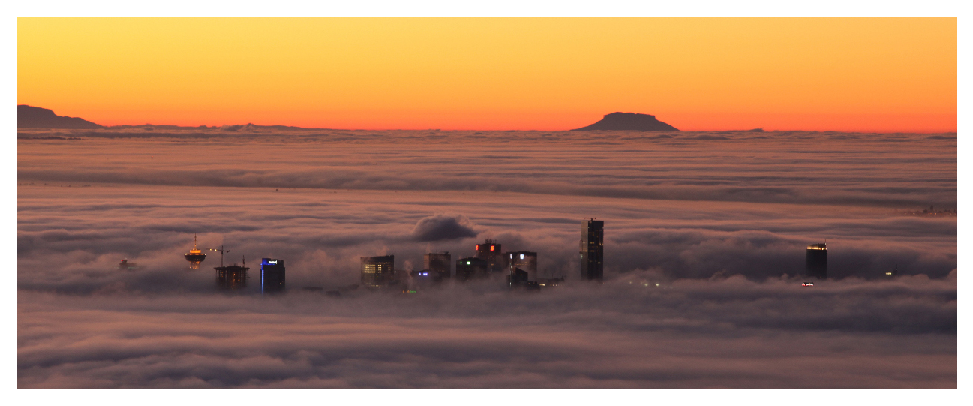
\includegraphics[width=16cm]{spoiler}
   \caption{Tweether showing the real time mood of Nebraska.}
  }

%% Uncomment below to disable the manuscript note
%\renewcommand{\manuscriptnotetxt}{}

%% Copyright space is enabled by default as required by guidelines.
%% It is disabled by the 'review' option or via the following command:
% \nocopyrightspace

%%%%%%%%%%%%%%%%%%%%%%%%%%%%%%%%%%%%%%%%%%%%%%%%%%%%%%%%%%%%%%%%
%%%%%%%%%%%%%%%%%%%%%% START OF THE PAPER %%%%%%%%%%%%%%%%%%%%%%
%%%%%%%%%%%%%%%%%%%%%%%%%%%%%%%%%%%%%%%%%%%%%%%%%%%%%%%%%%%%%%%%%

\begin{document}

%% The ``\maketitle'' command must be the first command after the
%% ``\begin{document}'' command. It prepares and prints the title block.

%% the only exception to this rule is the \firstsection command
\firstsection{Introduction}
\maketitle
%% \section{Introduction} %for journal use above \firstsection{..} instead

Weather affects our daily lives, from what we wear, what activities we do, what type of transportation we use, what we eat, or even how we feel.  With the increasing accuracy in weather forecasts people can gain an idea on the what type of weather they can expect for upcoming days. Activities are usually planned according to the weather outside (i.e. weddings) and alternative plans must be made in case of inclement weather. How people dress is also affected by weather; when the temperature drops people need to wear coats to stay warm. The economy is also greatly affected by the weather. Certain weather conditions can lower crop yield and cause higher prices in stores. Disastrous weather phenomena such as hurricanes, tornadoes, or even floods can cause devastation in communities resulting in homelessness, death, and destruction. Inclement weather can also cause delays in transportation on roads or for flights. We can also choose to ride our bike to work instead of driving the car if the temperature is warm enough. One thing that is an effect from all these items is how we feel.

\begin{itemize}
\item Are you sad that you can't enjoy the outdoors because it's raining?
\item Do you love that it's raining so you can bundle up and read your favorite book?
\item Do you love the snow because it's close to Christmas?
\item Do you hate the winter because you want it to be spring?
\end{itemize}

These feelings are all brought out by the weather outside. One person can feel positive about a certain type of weather and one person can feel negative. In this work we showcase a novel tool, named Tweether a visualization of real time Twitter and weather data to show the feelings of current users and how their emotions could fluctuate. Having the weather forecast up to 72 hours in the future, the emotions in current regions can be predicted. 

We see if the weather has any correlation to the majority of the population and we try to predict the future feelings of given weathers.  When thinking about warm and sunny weather we automatically assume majority of the population will be happier in comparison to dreary or cold temperatures. We plan to examine if majority of the population follows this pattern. We will also examine how the overall sentiment changes when we filter tweets so only tweets in regards to weather are displayed.

It is not enough to just determine the correlation between emotion and weather, but a novel visualization is necessary. Our work showcases a 3-dimensional map of Nebraska which highlights select clusters of weather. The correlation of tweets to weather is represented by line bundling. Introducing a clear relationship between weather and tweets the design presents a natural manner of representing correlation.


\section{Related Work}

Visualizations correlating sentiment and weather is highly sparse; the presence of live visualizations is also non existent. However, there are works showing the two portions of this work. Clustering of weather data has been done many times in the past. There is also vast number of visualizations which indicate sentiment of different locations.

\subsection{Psychological studies}

The natural correlation of weather with emotion has been studied profusely. \cite{bollen2011twitter,denissen2008effects,hannak2012tweetin,howarth1984multidimensional,lambert2002effect}  With various factors among the different research the conclusions attained were broad. Humidity, sunshine, and temperature have the greatest effect on mood. \cite{bollen2011twitter} 

In some research weather and mood, correlations have been debunked. There isn't consistency due to seasons and time spent outside. \cite{denissen2008effects} Having certain emotions regarding the season has strong links to seasonal affective disorder (SAD),  where people are depressed in regards to changes of the seasons, which usually occurs during the winter. However, most psychologists believe that the weather has an impact on psychological intentions. \cite{hannak2012tweetin} When observing serotonin levels in regards to sunshine there were strong relationships to being happy. \cite{howarth1984multidimensional} It has been found that weather may not play a big role in the positive attitude, but the negative attitude can have a correlation with weather. \cite{lambert2002effect}


\subsection{Social Media, Weather, and Emotions}

When dealing with the correlation of weather with emotion the research is fairly sparse. The works present use Twitter data for their social media feed and some form of weather data. However in comparison to our work the following research was computed on past data and used a 2-dimensional graph implementation to visualize the data.
 
Work has been done using two to four years of Twitter data and correlating it with meteorological data from NOAA. [3,6] Using urban areas in the United States as the area of interest, the tweets are passed to a sentiment analyzer that has a multi-level process. They first determine keywords which are identified from public events (i.e. entertainment or natural disasters), they then identify the mood state, and finally assign sentiment scores. To correlate the weather with the tweets they use a Generalized Mixed Model to display the non-linear relationship between emotion and weather. Using multiple variables for weather (temperature, temperature change, precipitation, snow depth, wind speed, solar energy, and hail) they determine the connection to hostility-anger, depression-dejection, fatigue-inertia, and sleepiness-freshness.  Their results indicate that the warmer temperatures create an angrier atmosphere, lower depression, and less sleepiness, and they determine the influence of temperature to mood is trivial. Their visualization is limited to graphs. \cite{hannak2012tweetin}
Other than using urban areas in USA we see relationships between temperature, humidity, and atmospheric pressure for one months tweets in the United States and weather data from Weather Underground. Using Linguistic Inquiry and Word Count for sentiment classification they saw a pattern with temperature and emotion of every state in the United States. Using regression analysis the find that the warmer states had a happier mood than the colder states. Their visualization was limited to a bar chart.

These works are limited in visualization and usability. Using past data is useful for our training and testing model however having a live view of what Twitter users feel in Nebraska is what we aim for in this work.


\subsection{Sentiment analysis in Social media}
Sentiment analysis is a topic that has been studied vastly. There are various methods to detect the sentiment of a sentence, however in regards to tweets we are not using complete sentences. Since tweets are limited to 140 characters the need to express oneself is limited to short meaningful phrases. We find abbreviations, neologisms, acronyms hashtags, emoticons and URL's throughout most tweets.

Certain features need to be extracted and some need to be filtered out. Filtering URL's, usernames, Twitter special words, and emoticons. \cite{keller2005warm} Stop words(i.e. “a”, “an”, “the”) are also removed due to not adding any extra sentiment information.  For classifying the tweets, a number of different methods are used, however the most prevalent one is Naive Bayes classifier. \cite{keller2005warm} Emoticons are used as basis for sentiment classification for classifying tweets as positive or negative in the training purposes. \cite{jain2010data,keller2005warm}

Using emoticons for classifying training data is novel, however, most tweets gathered in the live feed had a very low count of emoticons. So using that method was out of question. Filtering of URL's, usernames was used for our method as well. We also added to the filtering process to drop phrases beginning with hashtags.

\subsection{Visualizations}

\subsubsection{Clustering}
Clustering of data is a trivial task. However when introducing  temporal and time series data the task becomes non-trivial. Weather data needs to be clustered based on a value, proximity, and the changes throughout the given time span. There have been various visualization techniques for time series data. Visualizing time series data using spirals for large data sets is used to better identify periodic structures in data. \cite{pak2010twitter} Using wavelet to transform data along a multiresolution temporal representation to find clusters with similar trends is a useful method for exploring data in a time series fashion. \cite{li2014nasty} Using smooth data histograms for visualizing clusters in self-organizing maps is a simple method when using 2-dimensional data sets.\cite{pampalk2002using}

The mass majority of clustering visualizations use k-means clustering on the basis of their algorithms. \cite{li2014nasty,weber2001visualizing} We choose to follow this pattern as well. The user's dilemma of what clustering information is needed provides insight as to why k-means is widely chosen; primarily due to it being a simple clustering algorithm. \cite{weber2001visualizing}

\subsubsection{Bundling}
The correlation between various weather and sentiment partitions can be fundamentally represented as a graph. However, graph visualization remains a challenging task. A direct drawing straight lines for all edges can easily incur severe visual clutter, even with some optimization techniques, such as force-directed placement of vertices or clustering of vertices~\cite{KAUFMANN2001}.

To address this issue, Holen~\cite{holten2006hierarchical} proposed a concept of edge bundling that groups the related edges of a hierarchical graph together as a set of smooth curved bundles, and thus can significantly reduce visual cluster. Holen et al.~\cite{holten2009force} extended the original edge bundling method and presented force directed edge bundling (FDEB) for a general graph without hierarchy. Other researchers have also made similar efforts to generalize edge bundling~\cite{cui2008geometry,telea2010image,ersoy2011skeleton,gansner2011multilevel}. Few efforts have been dedicated to create extensions in 3D space. Lambert et al.~\cite{5571244} presented a 3D edge bundling to visualize geographical networks on the Earth surface. B\"{o}ttger et al.~\cite{bottger2014three} presented mean-shift edge bundling to visualize 3D functional connectivity across the cortical regions of brain. Their method combines FDEB and kernel density estimation edge bundling
(KDEEB)~\cite{hurter2012graph} with an improved numerical stability.

\subsection{Predictions}

Using the past Twitter data set it is necessary to predict the mood for the next days. Predicting the stock market based on Twitter mood has been studied. \cite{woodring2009multiscale} The notion that the mood of Twitter users can correlate to stocks immediately is not present, however, the mood is reflected when a few days have passed. Since the general public has strong connections with the outcome of a man-made entity there will be some form of correlation available. In our case, however, the weather is not a man-made entity, so finding a correlation between weather and mood, and then predicting the mood for the future can show zero correlations. We will address this idea later in this paper.




\section{Our Approach}

Implementing Tweether has multiple steps which are composed of individual and interconnected parts. The steps are illustrated in Figure \ref{fig:steps} . Tweether in its simplest form takes tweets and assigns a sentiment value which is then correlated to the nearest weather cluster. Each tweet is aligned to the map of Nebraska according to its location. The current hour visualization and the prediction visualization have the same user interface.

\begin{figure}[htb]
 \centering
 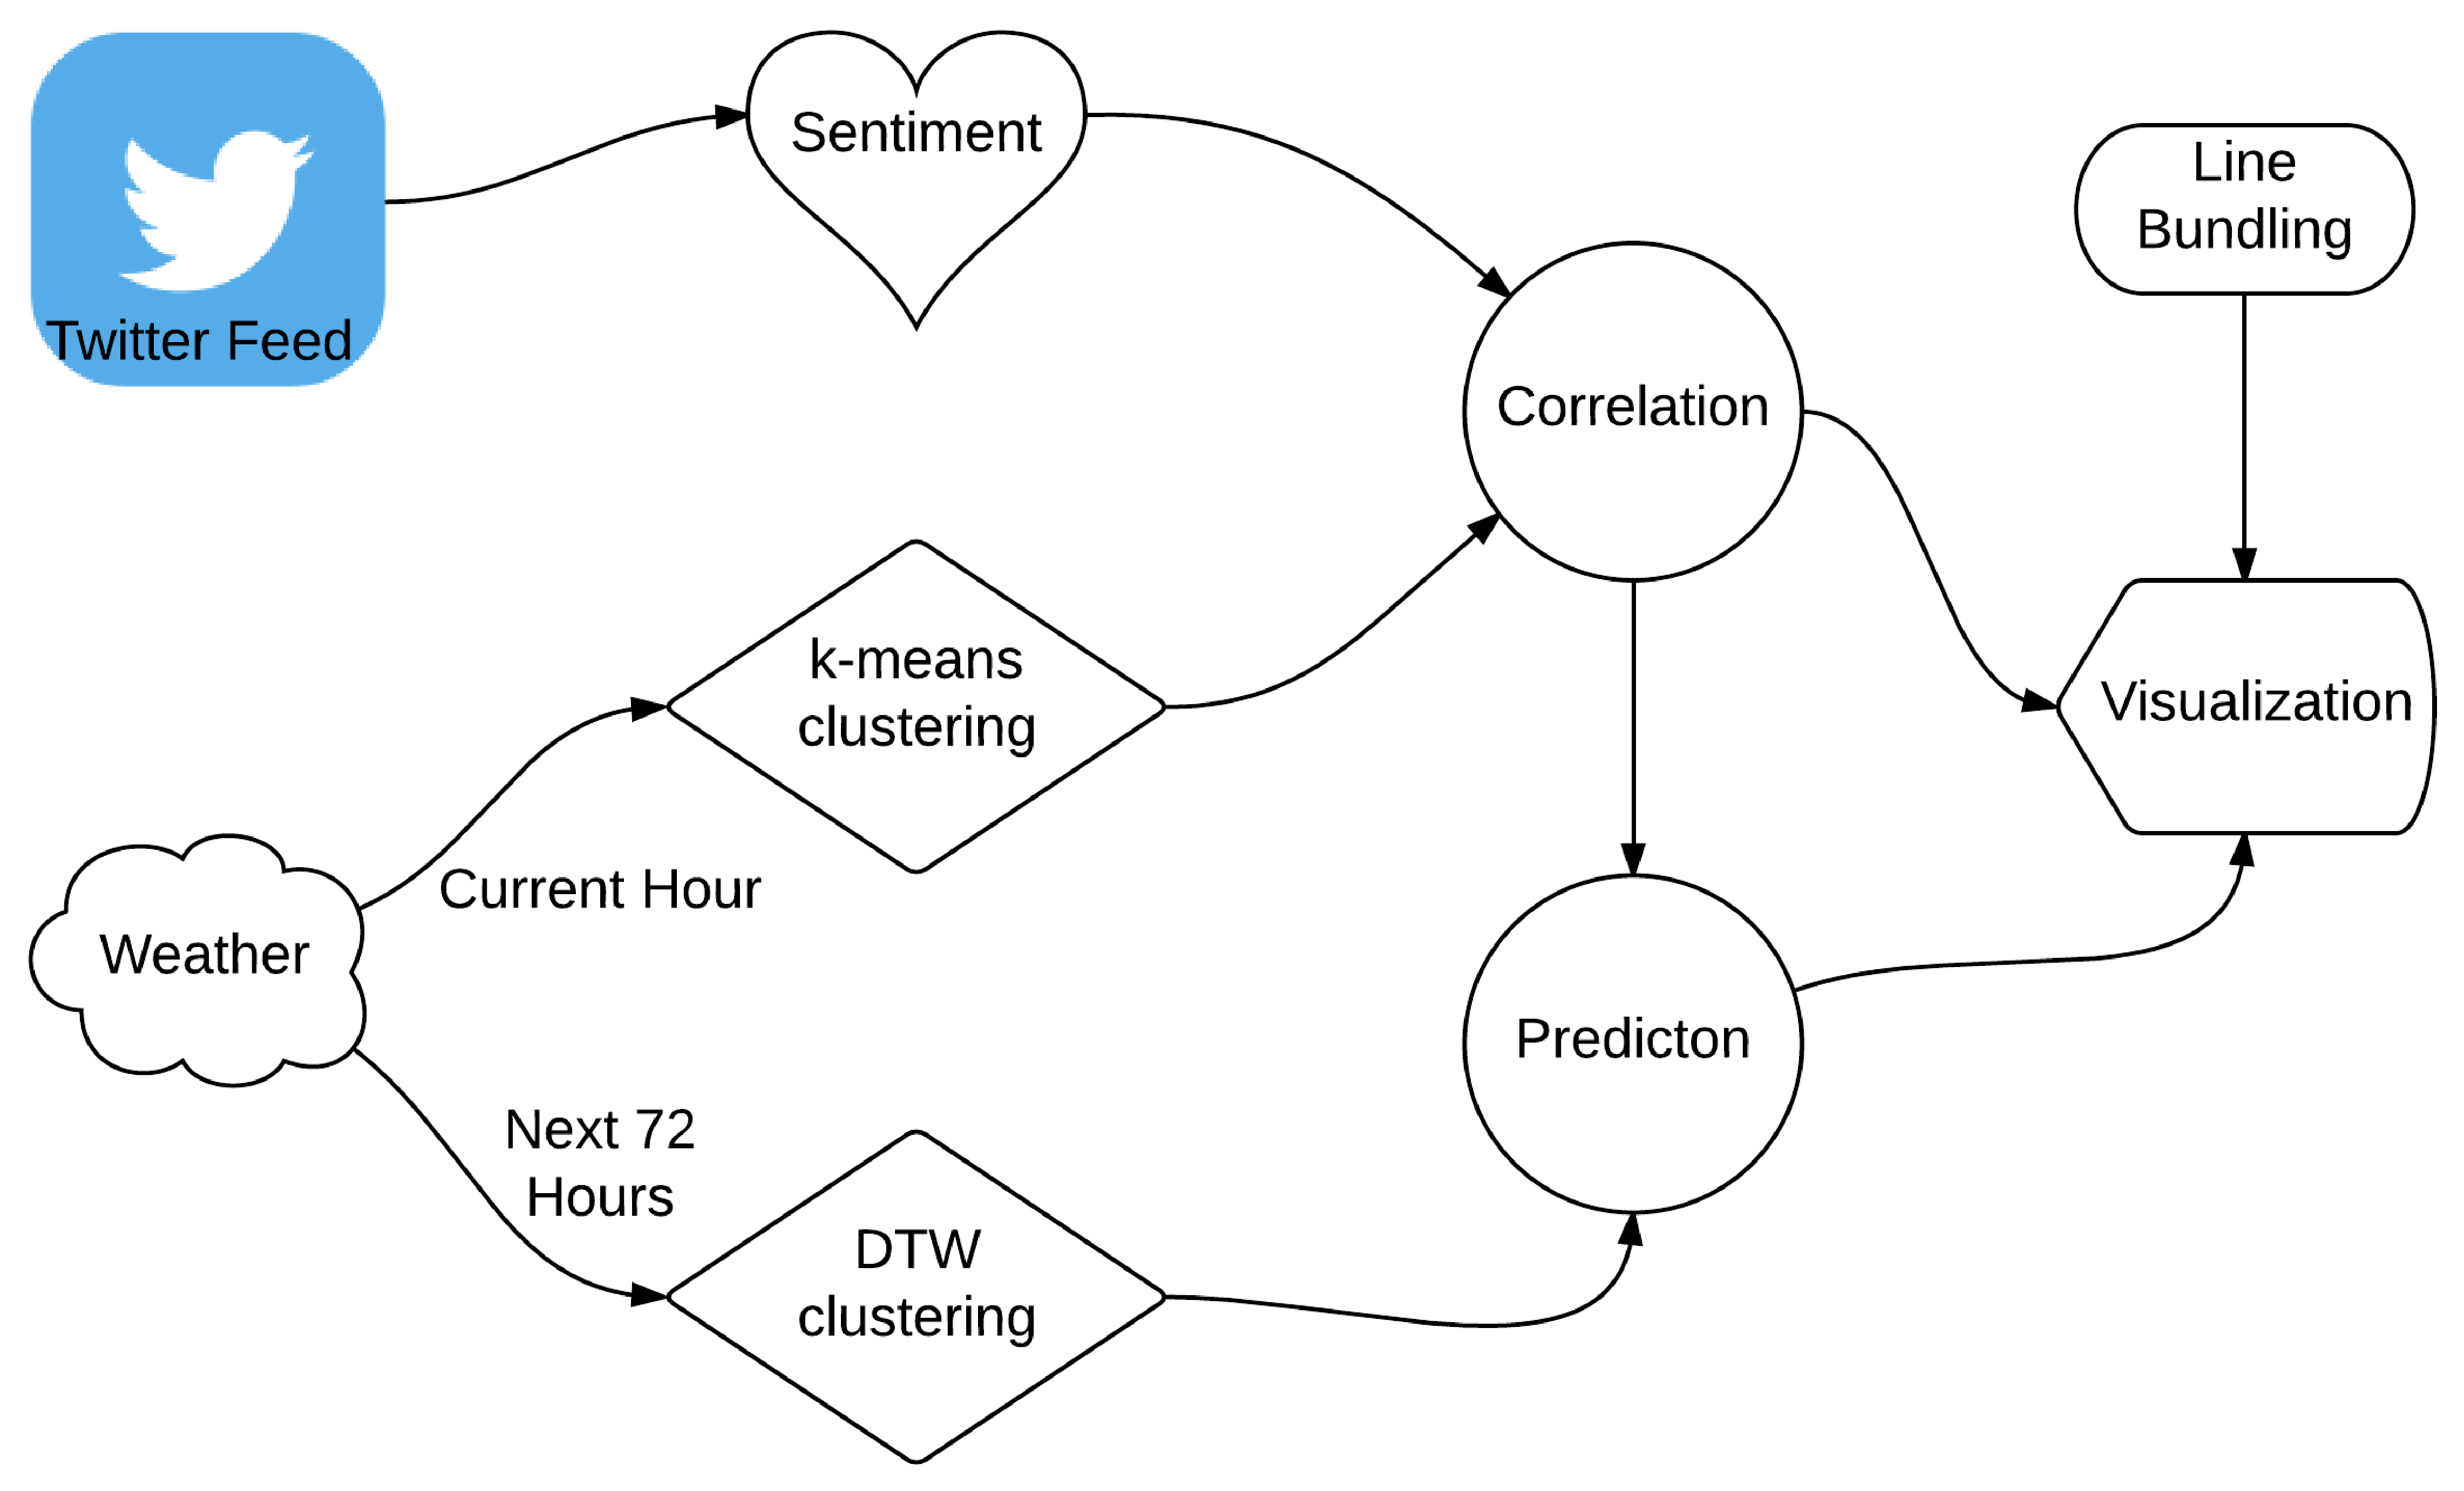
\includegraphics[scale=0.1]{steps}
 \caption{Steps of Tweether}
 \label{fig:steps}
\end{figure}





\subsection{Data Set}

There are two main data groups in this visualization. 

The weather data set is provided using the Weather Research and Forecasting (WRF) Model from the Holland Computing Center (HCC). The data is pushed every six hours with a forecast of up to 72 hours in the future. Each WRF file contains multiple variables in regards to weather (i.e. temperature, precipitation, wind speed, etc.). For this visualization, we choose to focus on the TSK variable which is related to the surface skin temperature. Each TSK file is represented via a two-dimensional array that is 34 x 24. The WRF file geographically corresponds to Nebraska and surrounding states as seen in Figure \ref{fig:maps}.

The Twitter data is the live data feed from Twitter users throughout Nebraska. Only users that have opted-in to use Tweeting With Location feature turned on are used. A geographic filtering process was used to use only select cities in Nebraska. Locations for the tweets are limited to the most populous cities in Nebraska (Omaha, Lincoln, Grand Island, Kearney, Fremont, North Platte, Norfolk, Columbus, and Scottsbluff). Since Nebraska has a fairly low population with most of the land being barren, only the most populous cities were chosen. The Twitter data is stored in JSON format where we need to extract the coordinates of each tweet and the tweet itself. Due to cities being on the border of Nebraska such as Omaha, the Twitter data needs to have a second filter which removes any tweets that don't have any relation with Nebraska.
\begin{figure}[htp]
  \centering
  \subfigure[Map showing surrounding states with counties]{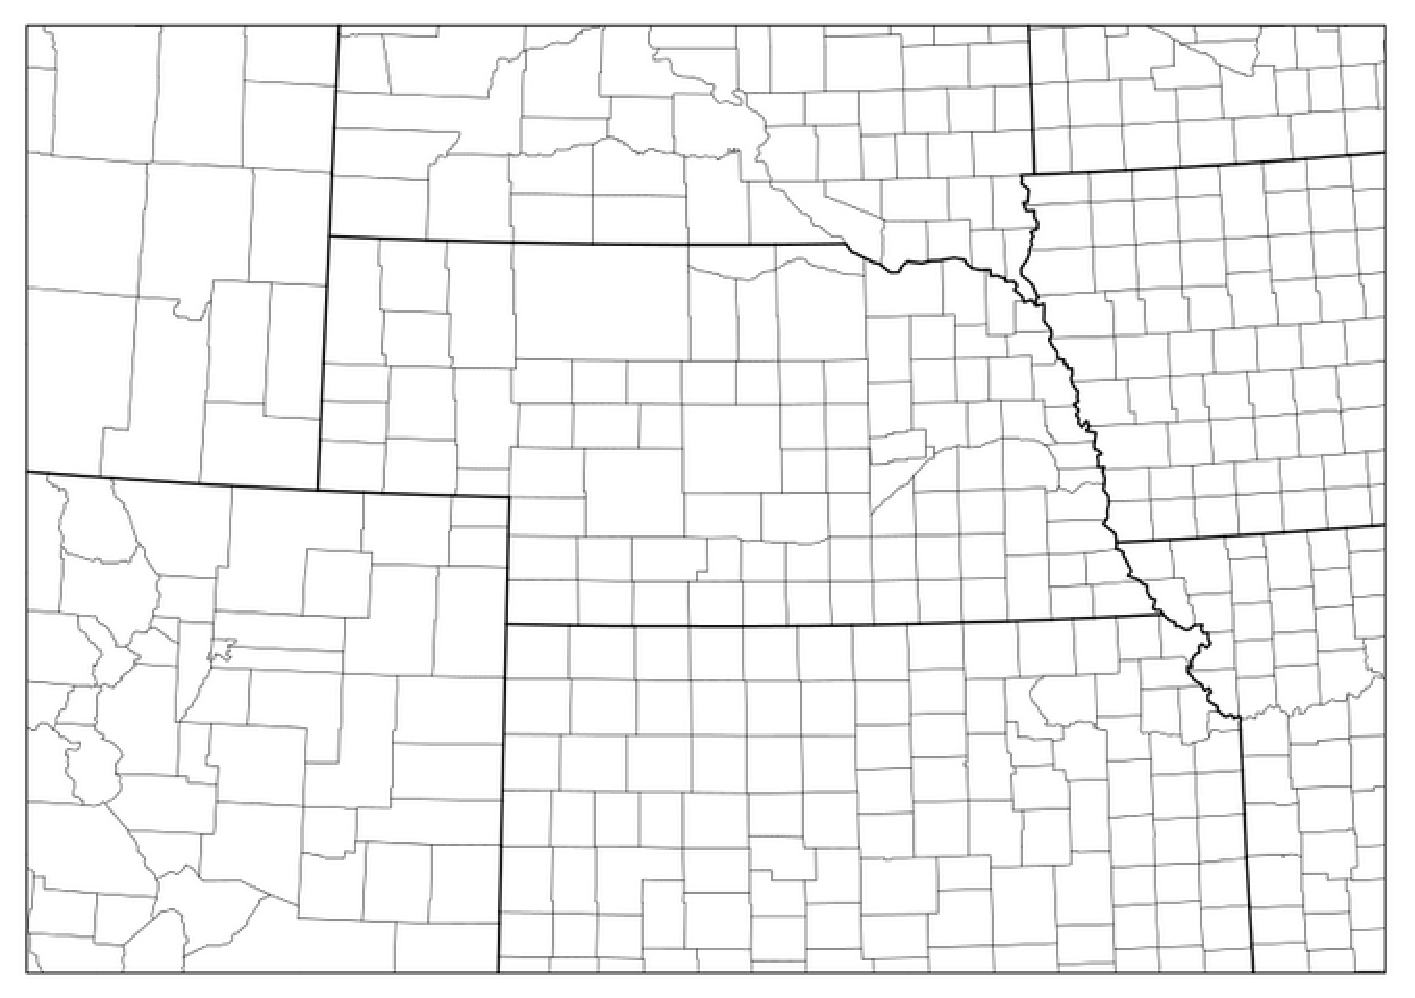
\includegraphics[scale=0.2]{mapBefore}}\quad
  \subfigure[Map reduced to show prominance to Nebraska]{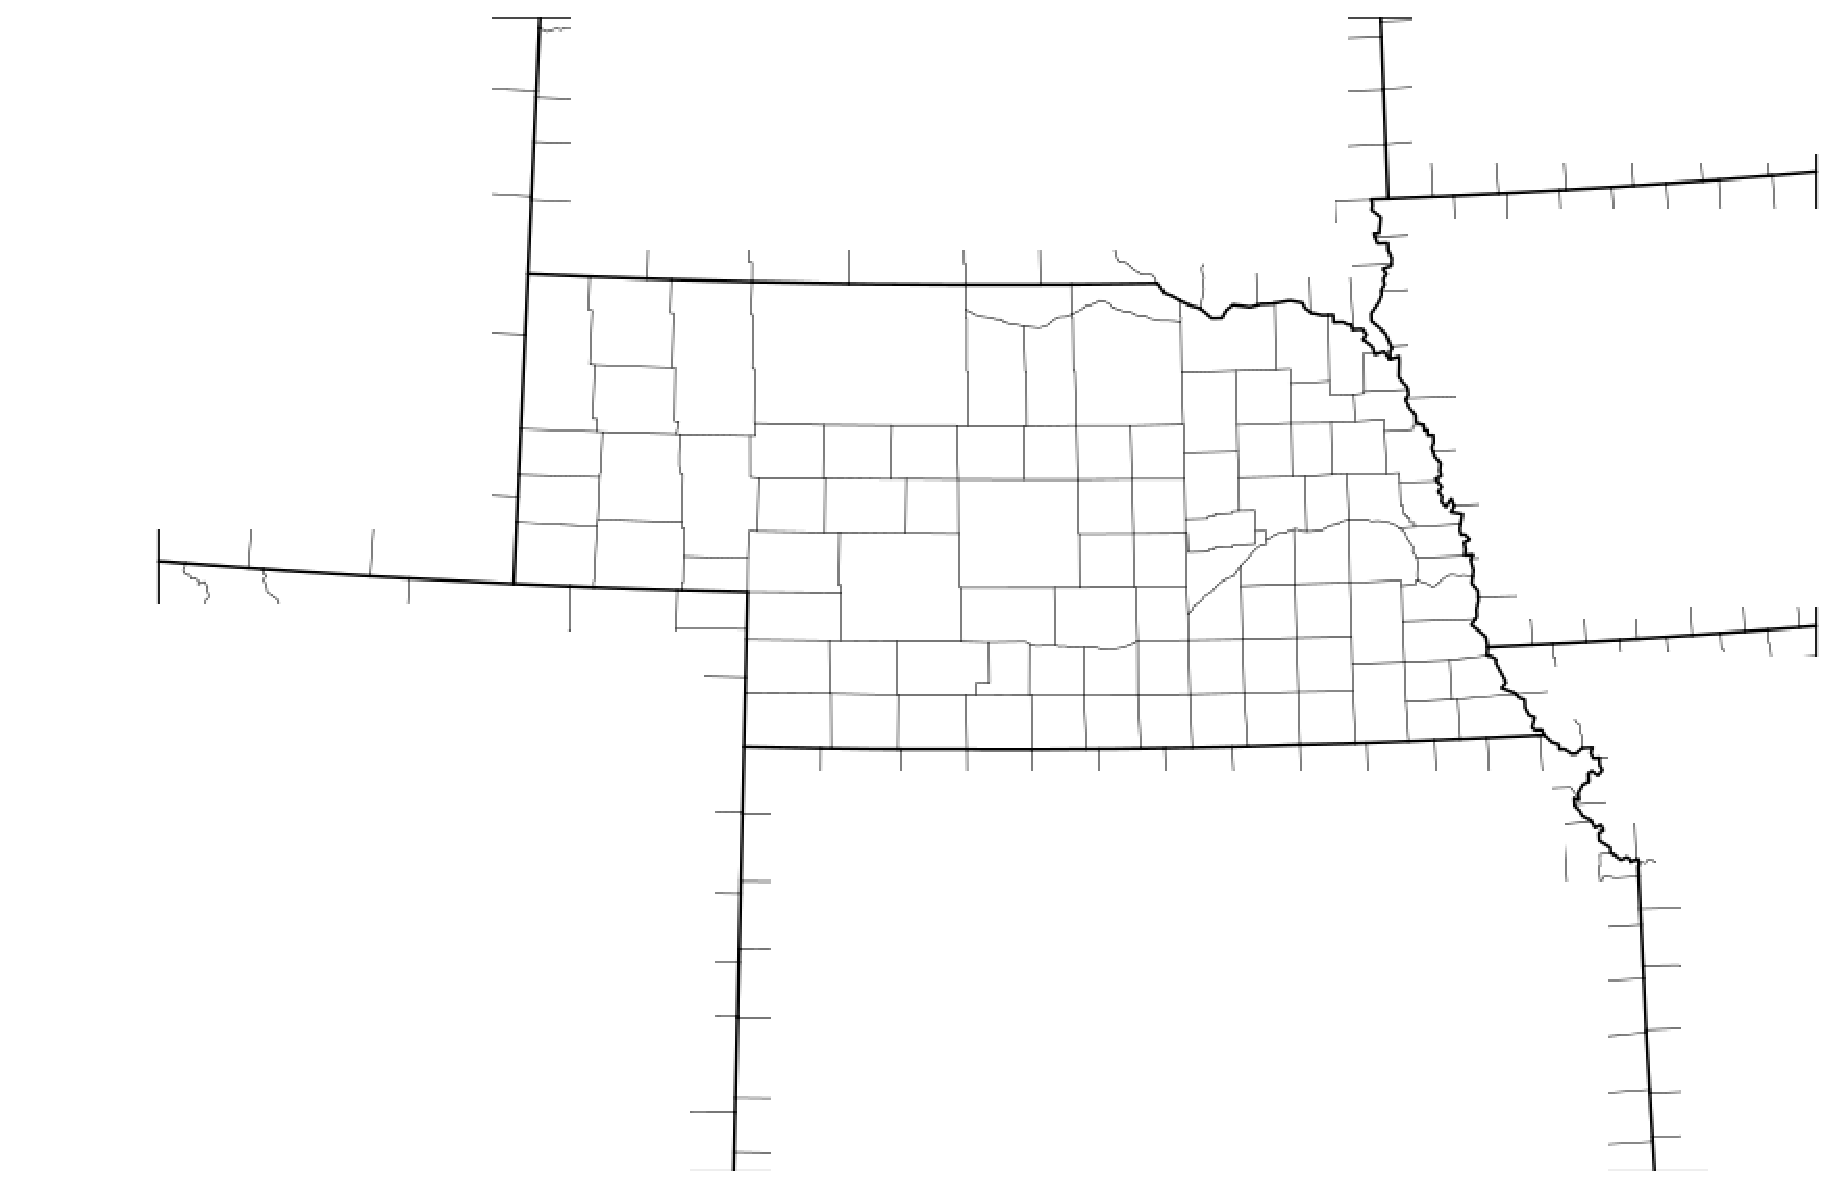
\includegraphics[scale=0.2]{mapAfter}}
\caption{Nebraska map before and after}
\label{fig:maps}
\end{figure}

\subsection{Clustering}
The clustering differs depending on if looking at the current hour or the predicted values for the next 72 hours. For the current hour, the k-means clustering algorithm is used. Since we don't need to worry about the future at the current state nothing additional is added to the algorithm. For predicted moods, we use the  dynamic time warping (DTW) algorithm.

The k-means clustering algorithm partitions the matrix of data into five clusters which can be dispersed. In the matrix, the dispersed clusters can create random patterns or create outliers. To remove outliers, they are filtered out creating fewer regions of the same cluster. The filtering process is based on the number of data points in each cluster. If there exists a cluster which has less than one percent of the overall number of clustered elements then this cluster is removed and the remaining data points which belong to a cluster are clustered again. This process is done as long as there exists a cluster which has less than one percent of the overall cluster count. 

For the forecasted weather, a modified k-means algorithm was used originally. Since k-means isn't very robust towards outliers due to adding a square weight on the value, we used dynamic time warping to measure the similarity between two hours. 

To smooth any randomness, connectivity is used to determine the percentage of surrounding elements with the same cluster value as the central element. If at least five out of 8 neighbors have the same value then this cluster is kept, otherwise the data point is removed. This method is repeated four times to ensure smooth clusters. The number of times to be repeated was chosen due to it creating the most smooth outcome amongst the majority of 73 hours.

\subsection{Semantic}

Each tweet can contain different attributes other than plain sentences. Due to each tweet being limited to 140 characters the majority of users tend to use abbreviations, neologisms (i.e. noob, troll), acronyms hashtags, emoticons, and URL's. Abbreviations, acronyms, and neologisms are taken into account for training our classifier, however, a few items are filtered from certain tweets. The filtering process removes  emoticons, URL's, usernames, and hashtags. In some situations, it is known that hashtags can provide instant insight as to what the users are feeling.[6] However, we feel with most hashtags that we encountered they contained useless text or sentences for tags instead of keywords.

A Naive Bayes classifier is used to determine the sentiment of tweets.
Using Robert Plutchik's theory, it states that there are eight basic emotions: 
\begin{itemize}
\item negative - fear, anger, sadness, depression, disgust
\item positive - joy, trust, anticipation, surprise
\end{itemize}
    
These emotions are the basic training portion of the classification of tweets. The synonyms for each category are taken into account and this sets up the basic foundation for the tweet classifier. 

Other than acronyms we also need to take into account profanity. The use of profanity in social media is very high and it may lead to a positive or negative emotion depending on the situation. To take into account how profanity is used in sentences, tweets were polled to see how these words were used. Using these tweets to train the classifier gave a pretty high accuracy rate in regards to profanity. In the beginning we tried to remove any tweet with profanity, however, this drastically lowered our tweet count. We then tried to remove occurrences of profanity in the tweet and use the remaining words as a judge of emotion. This worked in a few cases however for the most part the we believed that profanity gave insight to negative moods so we decided to take into account profanity.

Due to tweets using abbreviations and incomplete sentences, sentiment calculation is a nontrivial task. The classifier is trained using around 10,000 tweets, where each tweet was given a positive and negative score, and there were rare occurrences of duplicate tweet, and it was made sure that there was an equal portion of positive and negative tweets in regards to words where sentiment could go either way. 


\subsection{Correlation}
The correlation between each tweet and the cluster above is represented by a one to one mapping. As we see in Figure \ref{fig:clusters}(a), if there is a natural link then the mapping is pure. In situations where there isn't a direct link to any of the weather clusters the nearest cluster is used.

Other than the natural link between the primary cluster and the tweet we explore similarity of connections to other clusters regardless of the sentiment it may correspond to. This correlation is only available for the current hour. For each tweet, we use the top two relations to other clusters which we deem the secondary and tertiary clusters. Using the Pearson product-moment correlation coefficient, we determine the similarity of each tweet cluster to other clusters.(1) With a correlation value closer to one we keep the sentiment expressed in the primary cluster, however in the case of a correlation value closer to negative one we swap the sentiment expressed in the primary cluster. We look for the values closest to one or negative one and according to the sign we assign the proper sentiment value. Figure \ref{fig:clusters}(b and c) show the secondary and tertiary cluster.

\begin{equation}
\label{eq:pearson}
\rho_{X,Y}=\frac{cov(X,Y)}{\sigma_{X}\sigma_{Y}}
\end{equation}

cov is the covariance and $\sigma_{X}$ is the standard deviation of X \\

We use the location of the tweet and the temperature at that point to determine the best correlation value to all other points in other clusters. Disregarding the primary cluster we choose to focus on the mapping to the other clusters to indicate what other clusters the tweet could map to. In most cases the secondary and tertiary mapping have the same sentiment since the best fit is a cluster close by with a similar temperature. 


\begin{figure}[htp]
  \centering
  \subfigure[Primary Cluster]{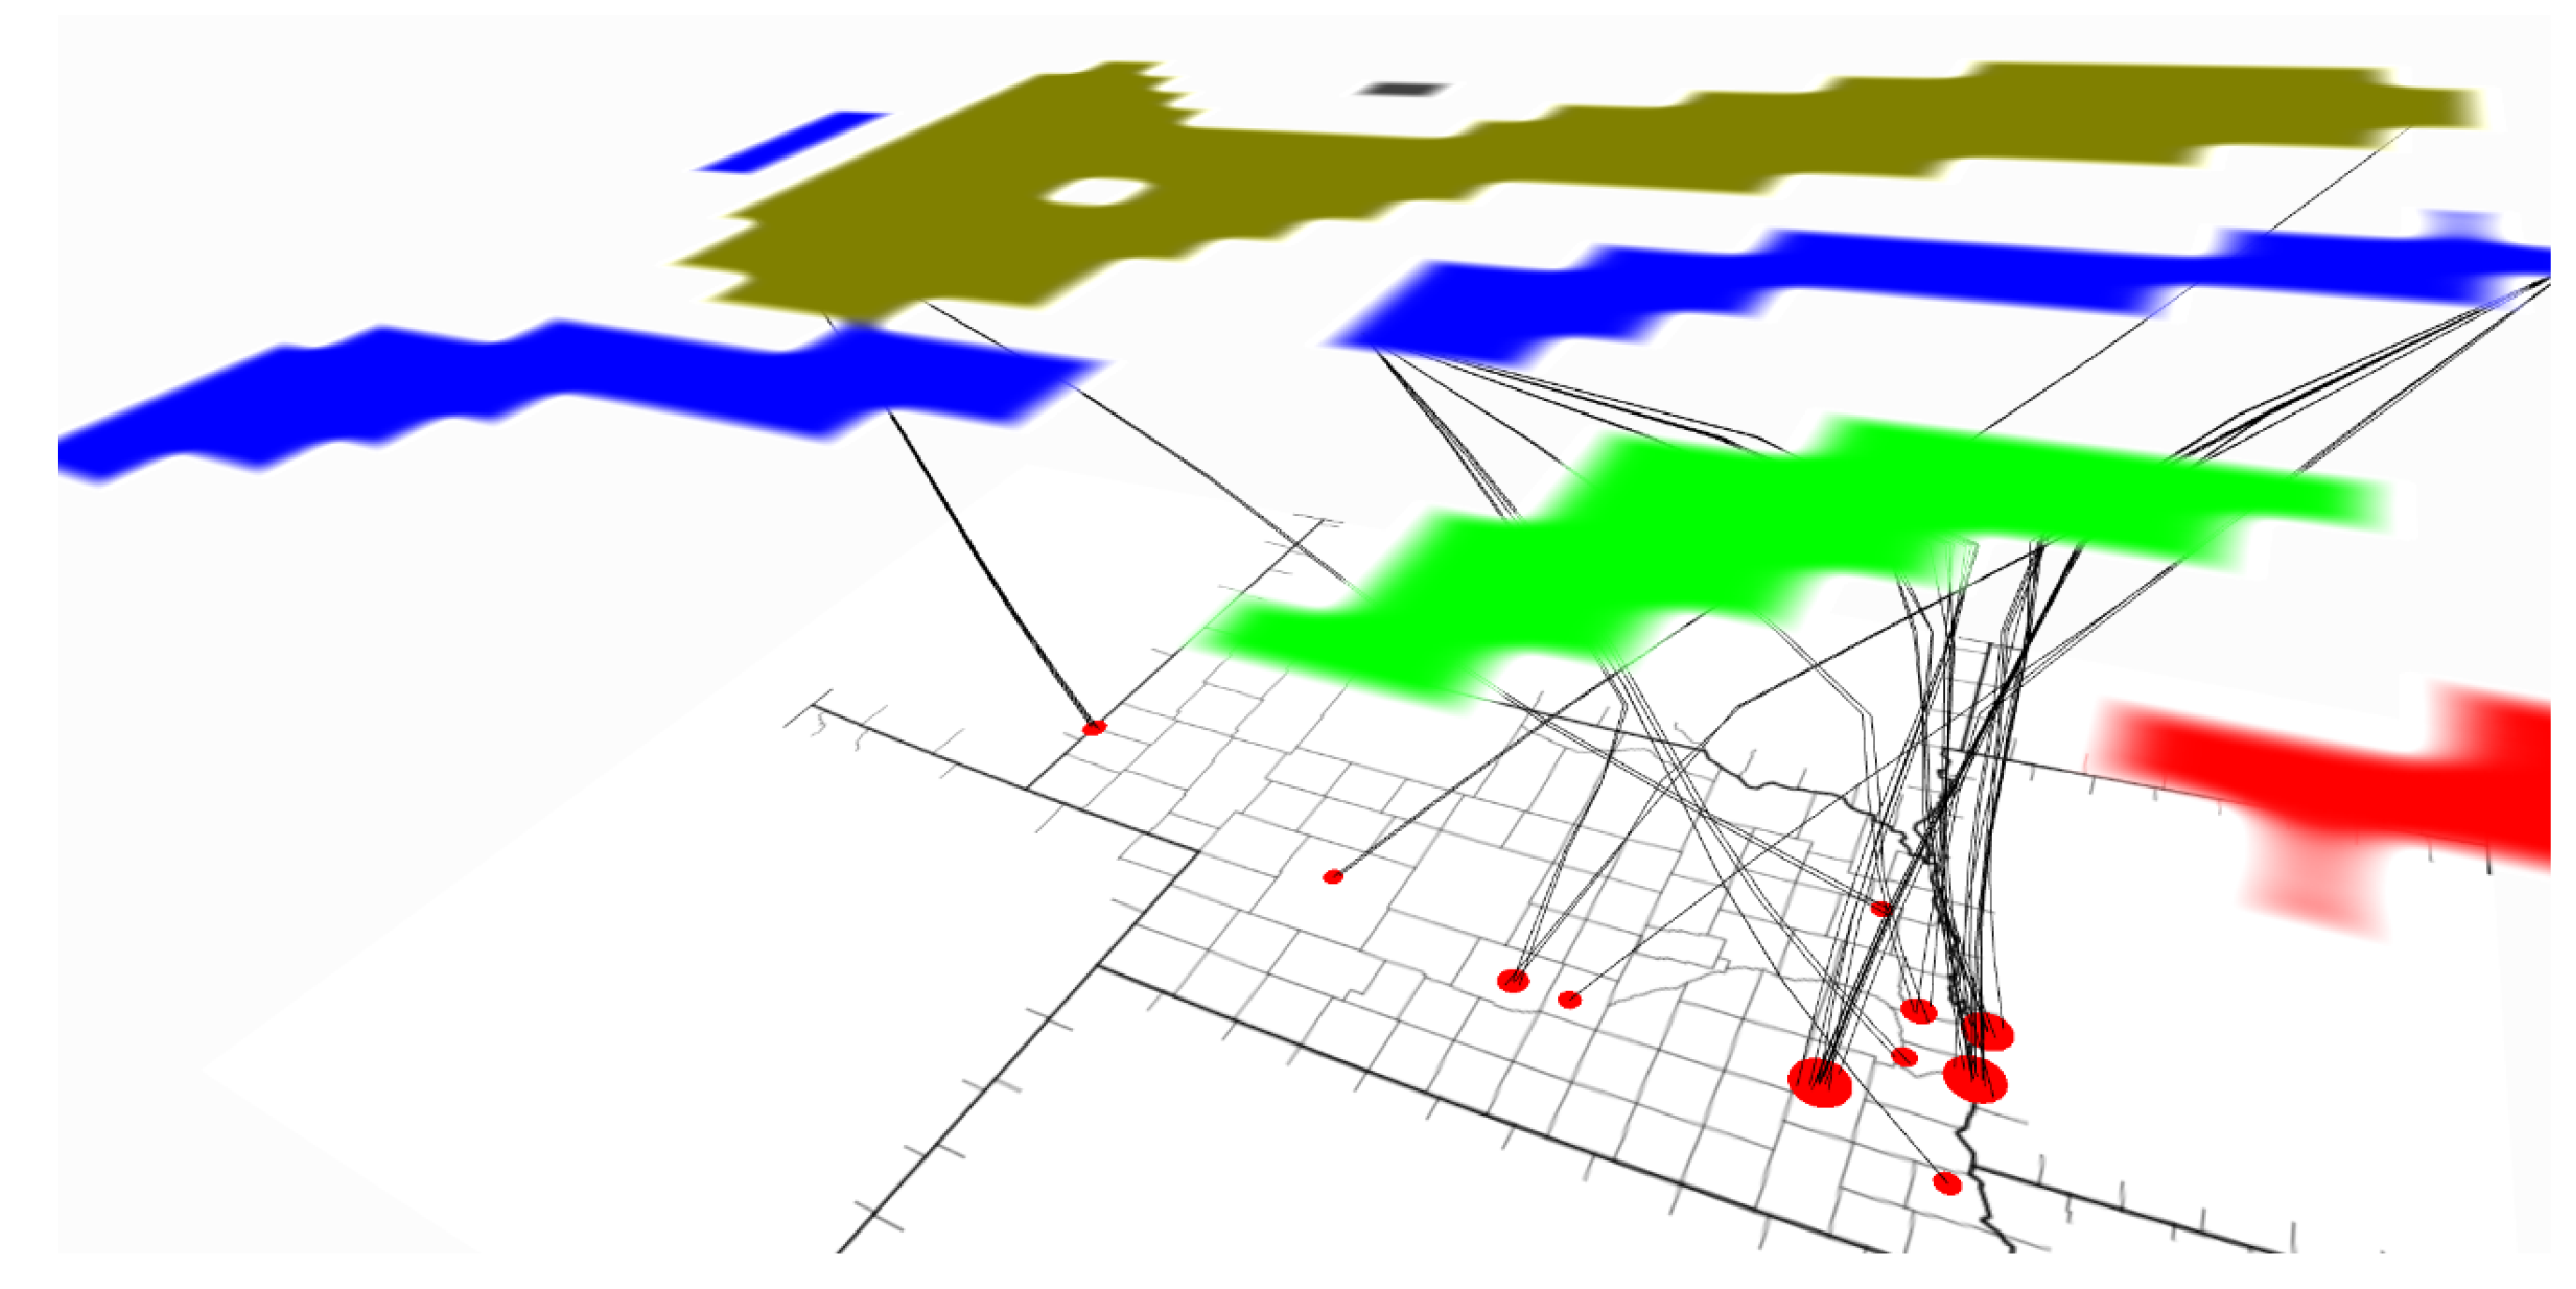
\includegraphics[scale=0.09]{blurBefore}}\quad
  \subfigure[Secondary Cluster]{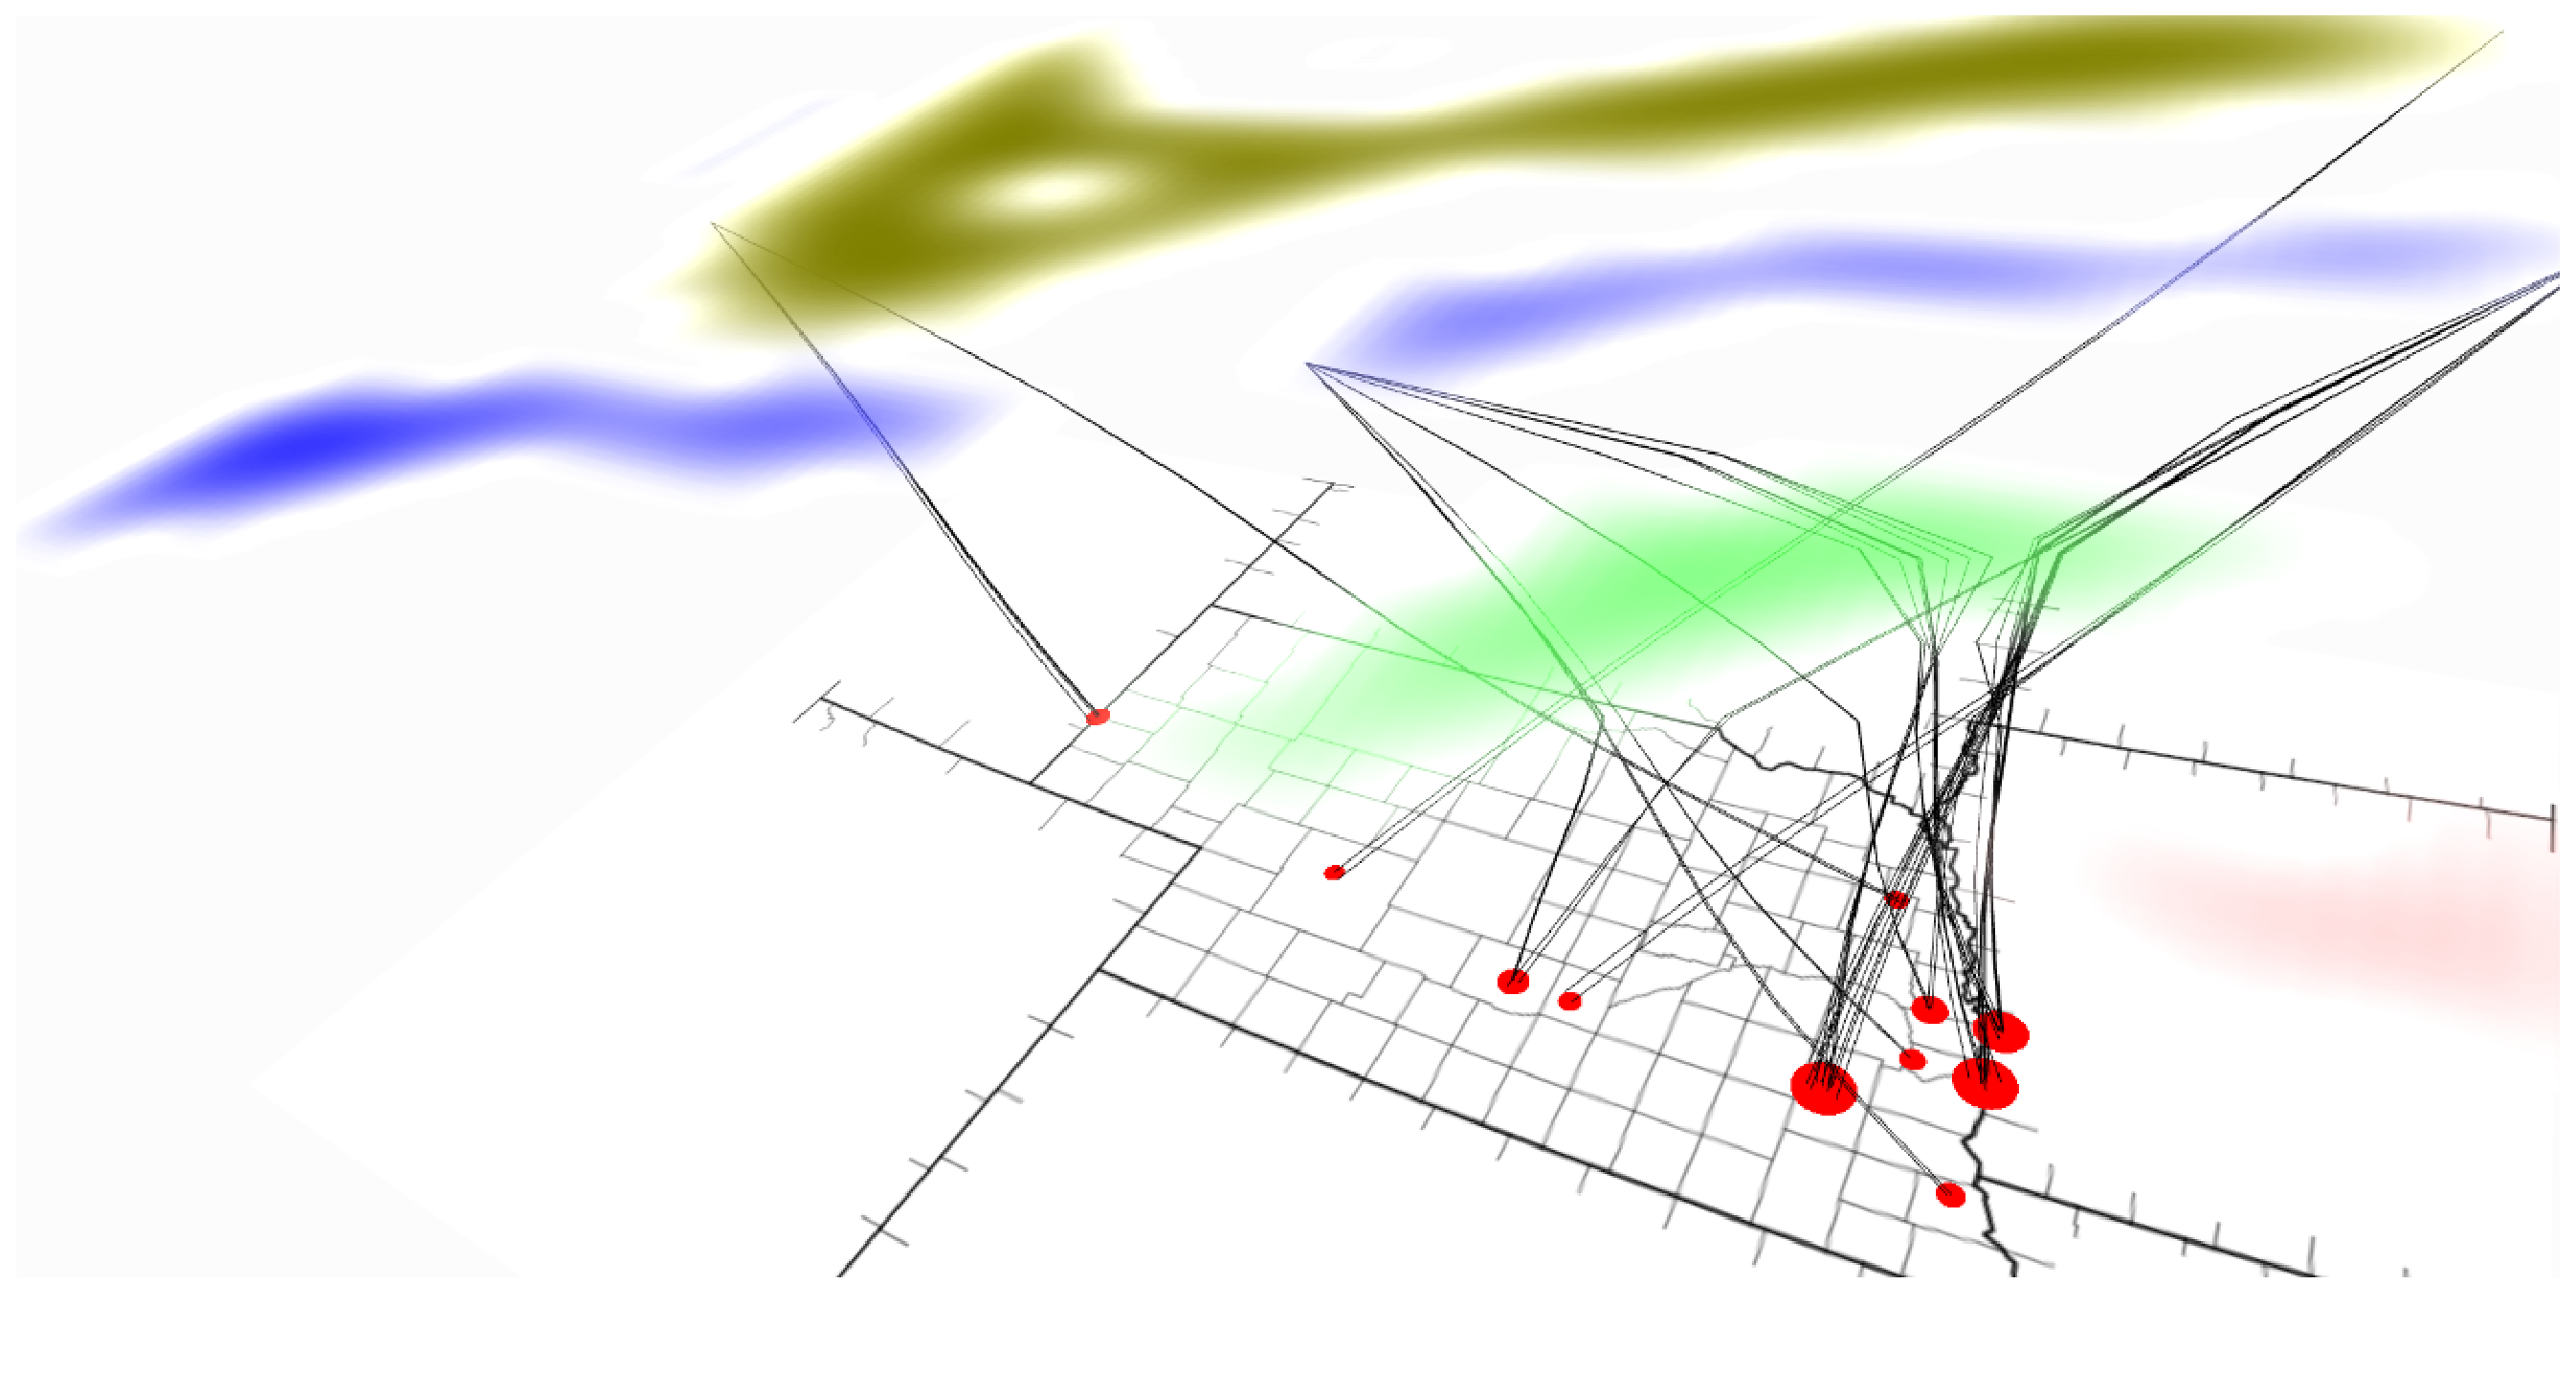
\includegraphics[scale=0.09]{blurAfter}}\quad
  \subfigure[Tertiary Cluster]{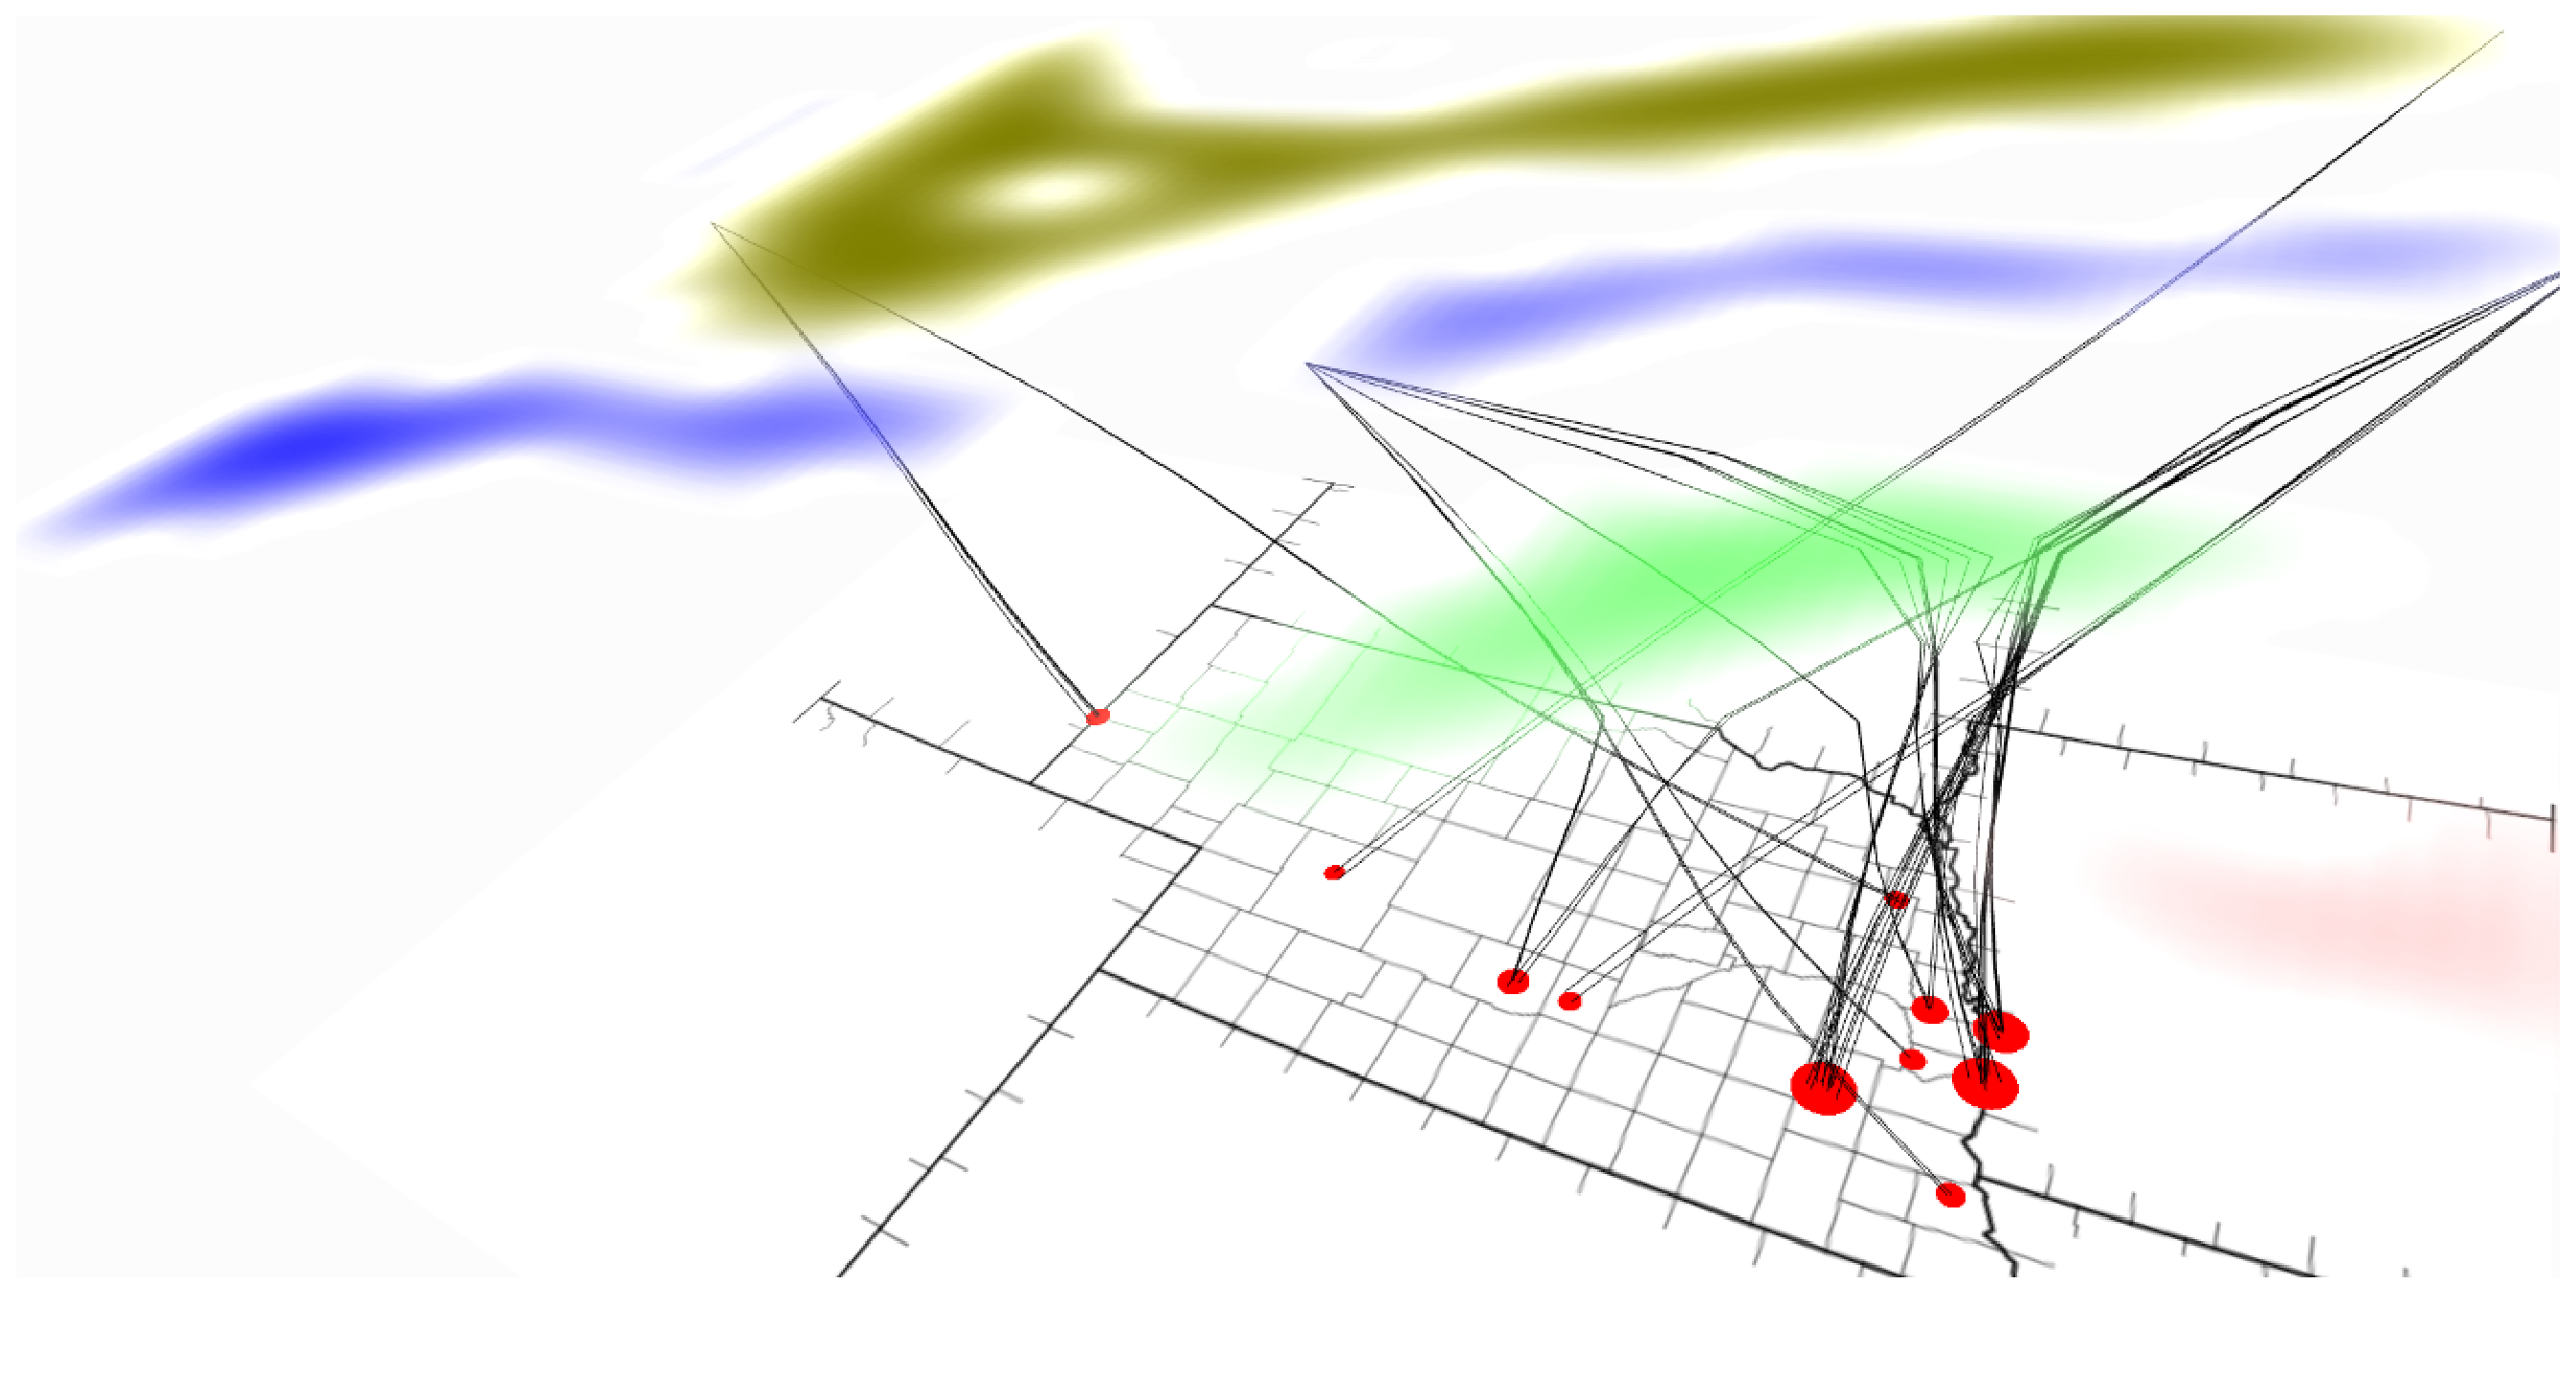
\includegraphics[scale=0.09]{blurAfter}}
\caption{Clustering of the weather. In this hour we see five different clusters. The blue cluster is seen in three different locations.}
\label{fig:clusters}
\end{figure}

\subsection{Line Bundling}

We adopt FDEB~\cite{holten2009force} to visualize the graph of correlation. We bundle the related edges with high compatibilities, and iteratively subdivide the edges to generate smooth curves with coherent shapes. This approach can effectively reduce visual clutter in 3D.

The original paper of FDEB~\cite{holten2009force} proposed four criteria, angle, scale, position, and visibility, for edge compatibility measures. In our design, as the edges are mostly oriented along the vertical direction between cloud and ground, the variation in angle or scale is relatively marginal compared to a general graph. In addition, as we display the edges in 3D, the visibility of an edge can be changed from different views. Therefore, only position (i.e., distance between midpoints of edges) is considered for computing edge compatibility in our design.

Similar to FDEB, we use an iterative simulation to refine the bundling. The simulation starts with $P_0$ subdivision points for each edge, and then preforms $C$ simulation cycles. During each cycle, a specific number of iteration steps $I$ is conducted to move the subdivision points to reach an equilibrium between forces. The number of iteration steps during the first cycle is $I_0$. After performing a cycle, the number of subdivision points is doubled to smoothen the edges, and the number of iteration steps $I$ is decreased by a factor $R$. We found that a configuration of $P_0=1$, $C=6$, $I_0=50$, and $R=\frac{2}{3}$ leads to appropriate results in our design. 


\subsection{Prediction}
Predicting the future is mostly based on facts. We have at our disposal the current mood and the current temperature, all of the previous days tweets and the temperatures for each hour, and the predicted temperature for each hour for the next two days. Using these facts we try to determine what the sentiment at each location which people are tweeting from currently will be for the next two days. 

Determining the mood of the current locations up to 72 hours in the future is a nontrivial task. Our prediction technique is completely based on the current hour and the previous day. We choose not to use data from earlier times since the trends today are definitely not the same a year ago let alone a month ago. In addition to this, we should state that the weather is unpredictable for the state of Nebraska.

We started with the most rudimentary implementation, by solely comparing which number is closer by simply comparing the difference. If the current temperature is closer to the predicted temperature then the sentiment for the current hour is used to show the prediction. If the sentiment of the hour we are trying to pick has a closer temperature to the same hour from the previous day then we use the sentiment from the previous day. 

Seeing that the previous stated implementation was very crude we tried a different method. Depending on the hour we are trying to predict we state that if the current hour is at most five hours ago we will place a higher weight on using the current hours values, however when going past five hours we place more weight on the previous days values, where the further we are from the current hour the less weight it plays. Using this method we take the sentiment based on the percentage from the weight.

The final method we try is a combination of above methods. Where we first determine the closest temperature value to the hour we are trying to predict the sentiment. Then based on the difference we determine the weight the two different sentiment sets place \eqref{eq:w}. As we see in \eqref{eq:p} X and Y represent the current temperature and the previous day's temperature respectively, and Z represents the temperature of the hour that we are trying to predict. The number of good and bad sentiment lines is calculated in \eqref{eq:gb}, where $G$ and $B$ represent the number good and bad tweets predcted by using the good and bad tweets of X and Y. The details regarding how well the different methods performed will be seen later on in the case studies.\\

$p_1$ and $p_2$ represent the difference between the temperatures
\begin{equation} \label{eq:p} p_{1}=\left | Z-X \right |	\qquad p_{2}=\left | Z-Y \right |	 \end{equation}

$w_1$ and $w_2$ represent weight of the temperatures
\begin{equation} \label{eq:w} w_{1}=\frac{p_{2}}{p_{1}+p_{2}} 	\qquad w_{2}=\frac{p_{1}}{p_{1}+p_{2}}   \end{equation}

$g_x, g_y, b_x,$ and $b_y$ represent the amount of good and bad tweets in X and Y
\begin{equation} \label{eq:gb}  G = g_{x}w_{1} + g_{y}w_{2}	\qquad B = b_{x}w_{1} + b_{y}w_{2}	 \end{equation}



\section{Visualization}
The novelty of this work is pictured through the 3-dimensional visualization. The visualization is comprised of multiple layers where there is a natural visual connection between the layers. Many different methods could represent this data correlation however, we have created a novel visualization. The layers are connected via line bundles to dictate how the majority of the Twitter users in Nebraska are feeling.

\subsection{Layers}
The visualization is represented by three main layers. The base layer contains the map of Nebraska and neighboring states. We have chosen to show the counties in Nebraska to gain insight on the population distribution in the state, however we choose to keep the other states plain to indicate emphasis of correlation to Nebraska as shown in Figure \ref{fig:maps}.

On the map of Nebraska, there are circles which indicate the area that Twitter users are posting from. The radius of the circle corresponds to the amount of people posting tweets in the vicinity. Using the WRF data set for the longitude and latitude values for the map, we obtained the intermediate values via interpolation. For each tweet location, the euclidean distance is calculated to get the nearest longitude and latitude location.

The middle region contains the line bundles which starts from the Twitter user location and ends at the weather cluster they correspond to above depending on the sentiment. The topmost layer is the weather clusters.

The middle region contains the line bundles from the Twitter user location to the weather cluster they correspond to above depending on the sentiment.The topmost layer is the weather clusters.

\begin{figure}[htp]
  \centering
  \subfigure[Before blurring]{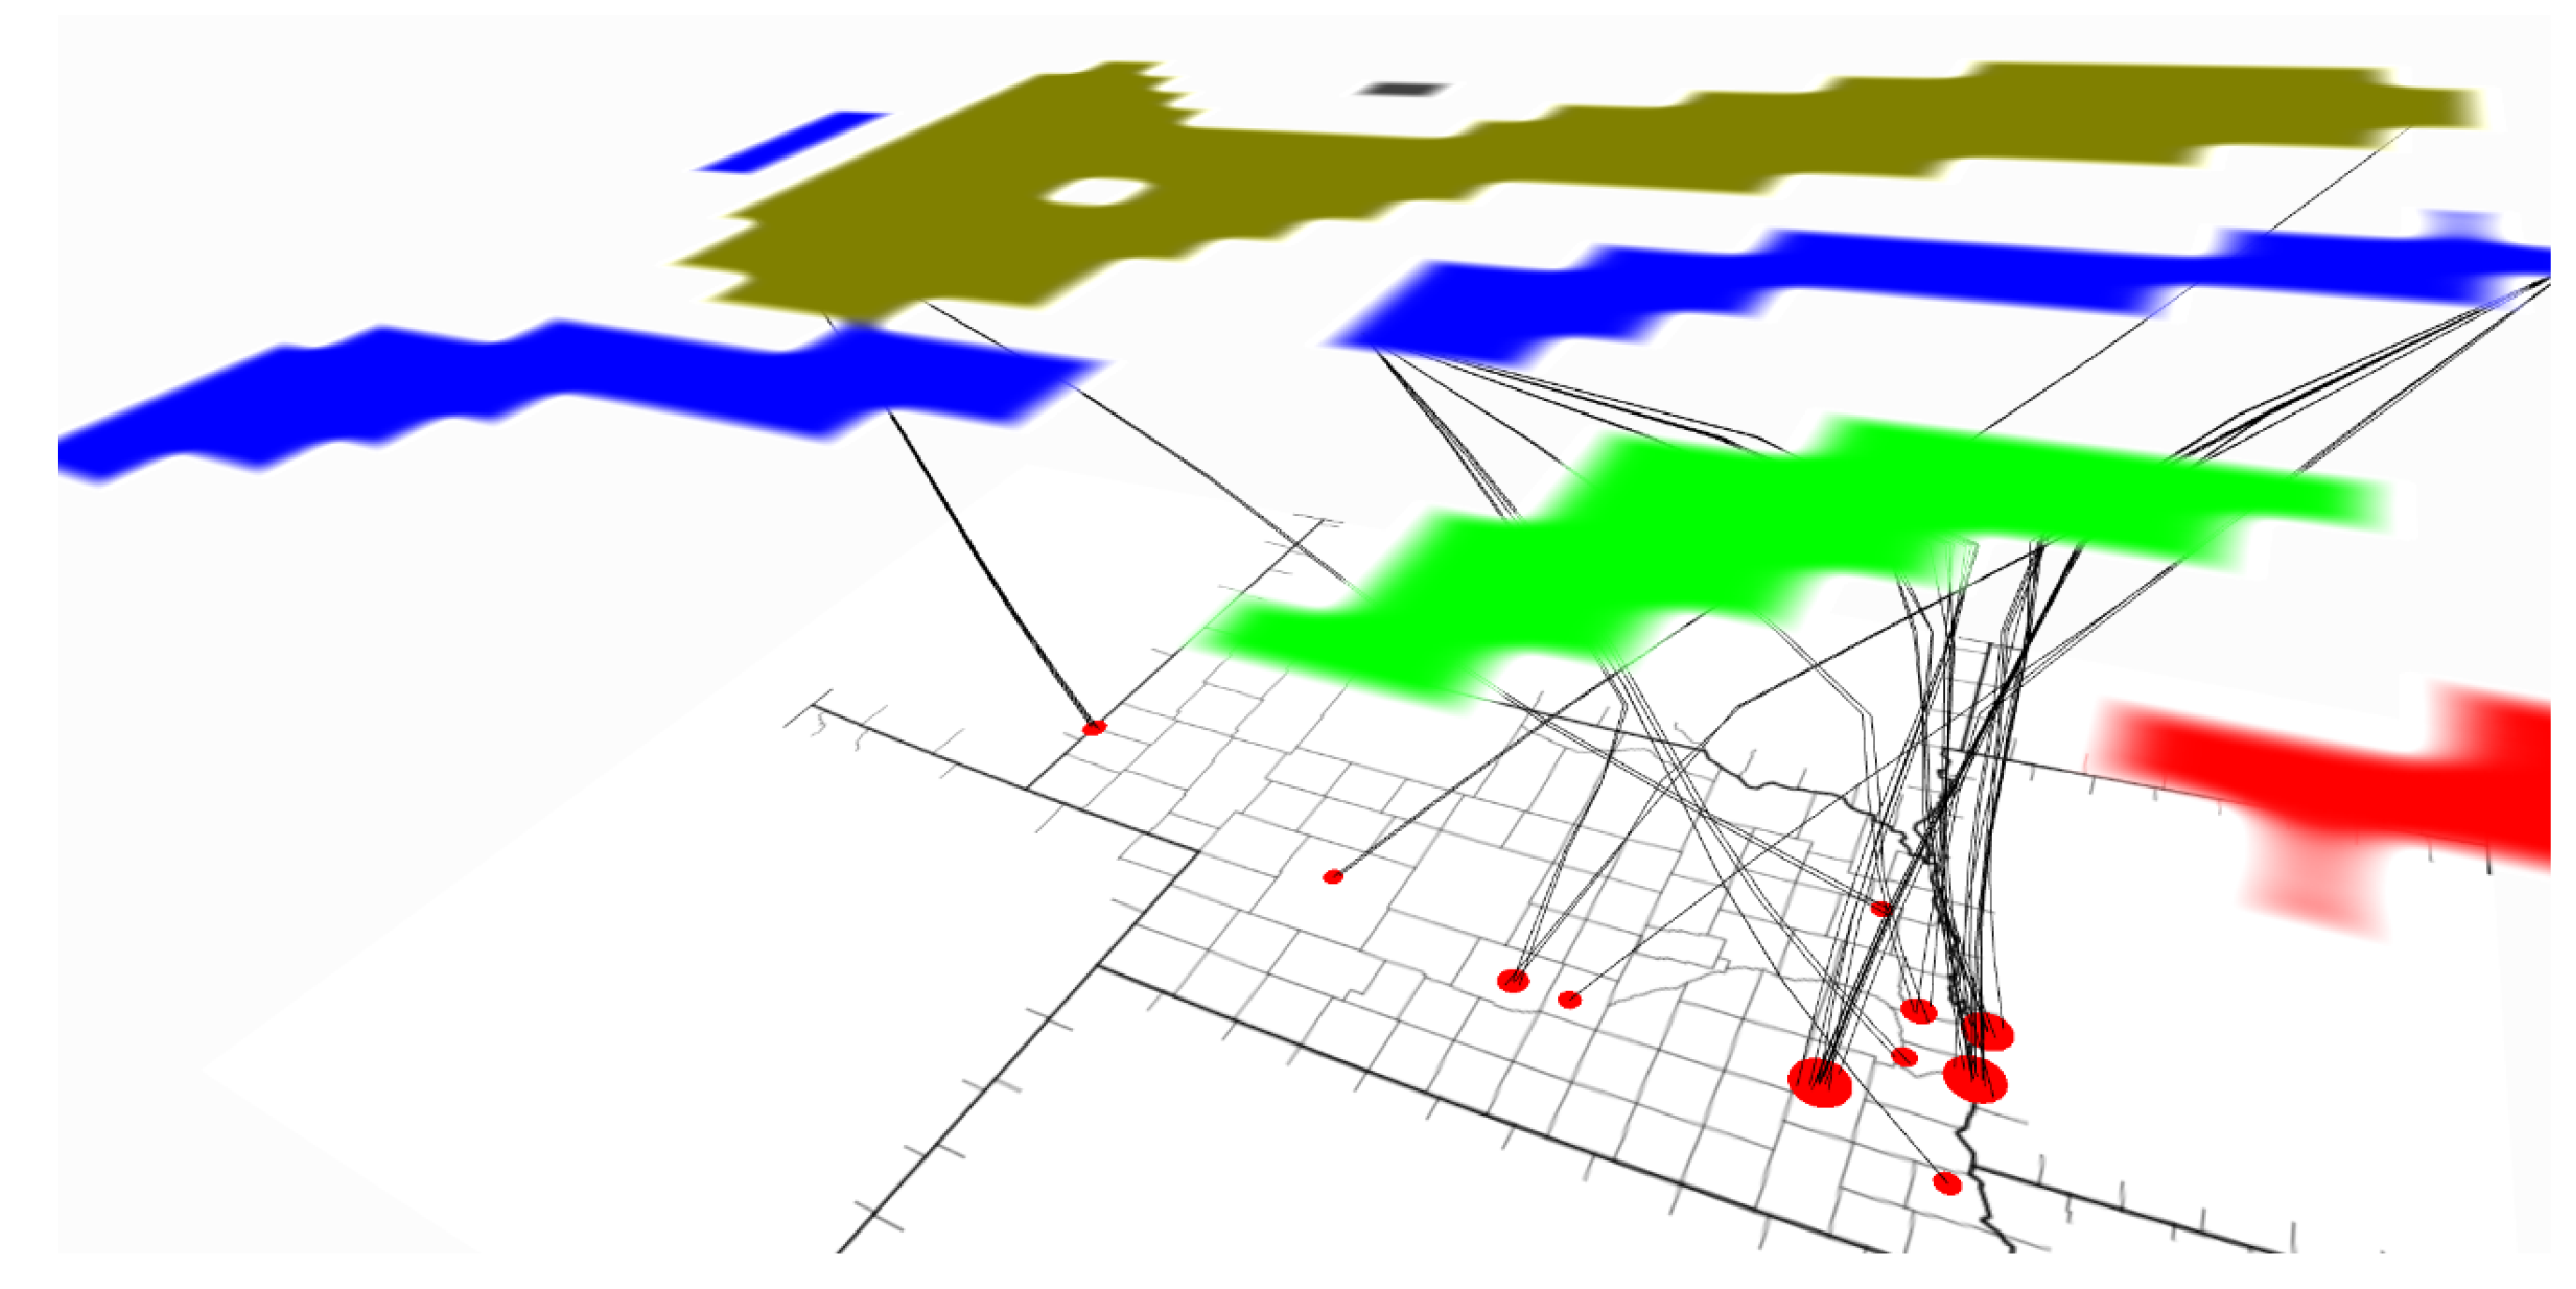
\includegraphics[scale=0.09]{blurBefore}}\quad
  \subfigure[After blurring]{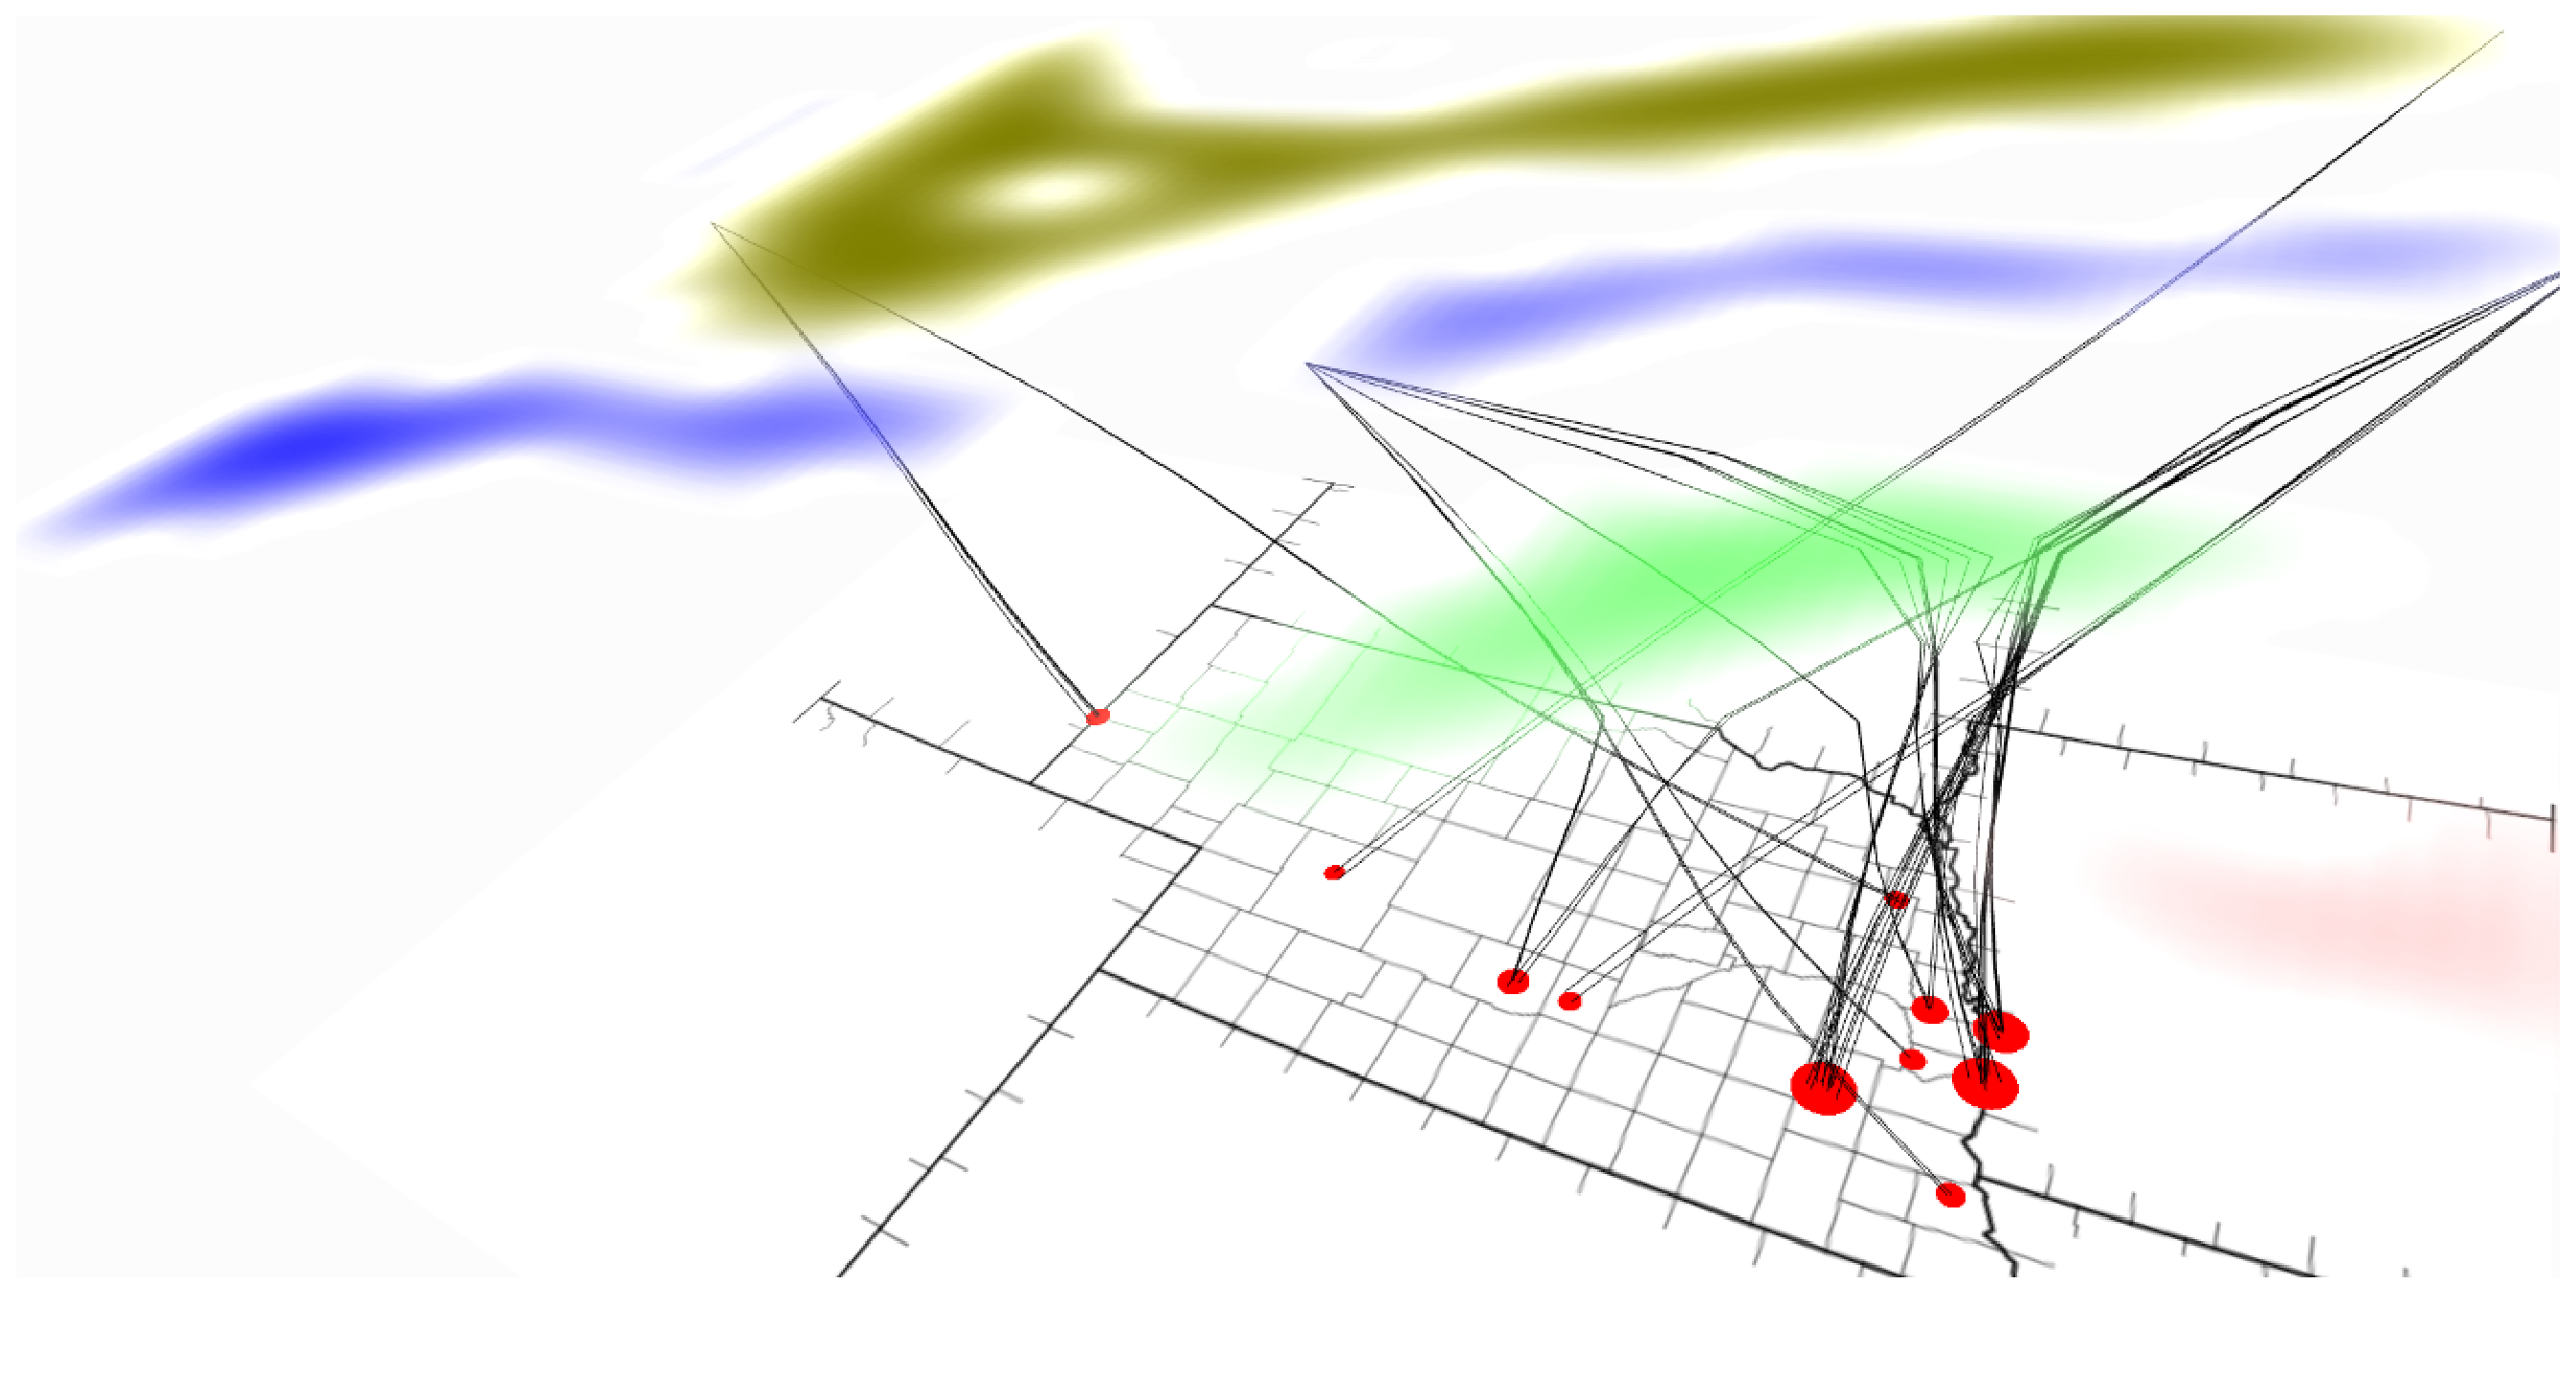
\includegraphics[scale=0.09]{blurAfter}}
\caption{Clustering of the weather. In this hour we see five different clusters. The blue cluster is seen in three different locations.}
\label{fig:blur}
\end{figure}

\subsection{Cloud Reperesentation}
Each cluster is represented by a different color. Clusters which aren't connected of the same color indicate the same conditions in other locations of Nebraska as seen in Figure \ref{fig:blur}.

Once the cluster for each hour was attained we needed two edge points for the data to link up to. These two edge points correspond to positive and negative emotions. We had different ideas on how the points should be picked. At first we were thinking to give half of one cluster to the positive emotion and the other half to negative emotions. This method seemed like a good idea at the beginning however in the visualization the output looked cluttered as seen in Figure \ref{fig:corners}(a). The second method we tried split the cluster in half and used the center points of the two half's. This was also a good idea until we came into situations where the cluster was represented by a very small amount of data points causing the visualization to look awkward. (Figure \ref{fig:corners}) We finally decided on a method where for each cluster the positive tweets would map to top rightmost point in the cluster and the negative tweets would map to the bottom leftmost point. This reduced visual clutter and helped in situations where the cluster size is fairly small. (Figure \ref{fig:corners})

In our visualization, the clusters appear as clouds. Initially, we had the user space and the weather space flipped, however, we believe that the way we present the data is novel and more intuitive. Each cluster is blurred at the boundaries to make the graphical interface cleaner and aesthetically pleasing as seen in Figure \ref{fig:clusters}(b).




\begin{figure*}[htp]
  \centering
  \subfigure[Half good half bad]{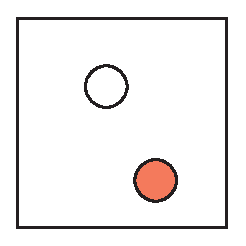
\includegraphics[scale=1.5]{sample}}\quad
  \subfigure[Half good half bad centers]{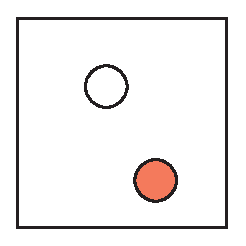
\includegraphics[scale=1.5]{sample}}\quad
  \subfigure[Corners]{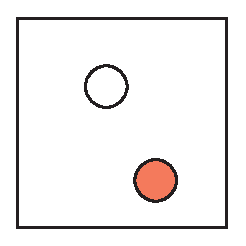
\includegraphics[scale=1.5]{sample}}
\caption{Determining the best position for indicating negative and positive tweets in the cloud clusters.}
\label{fig:corners}
\end{figure*}

\subsection{Line Bundling}
Each bundle is composed of multiple lines where each line represents one tweet. Every bundle represents positive or negative sentiment. The sentiment is represented in two ways. Depending on which corner the bundle is linked to indicates the sentiment, also the more intuitive notion is the color of the bundle. Naturally we associate the positive sentiments to the green bundles and the negative sentiments to the red bundles.

The opacity of each bundle represents the intensity of the correlation between the cluster and the tweets. The bolder the line the stronger the relationship between the two points is. The primary cluster has a stronger hue in comparison to the secondary and tertiary clusters. Both of these links will have a staggered decrease of intensity of color. Thus, we state that the more prominent the link between the tweet and the cluster the higher the opacity of the line.


\begin{figure*}[htp]
  \centering
  \subfigure[Temperatures in Omaha and Lincoln]{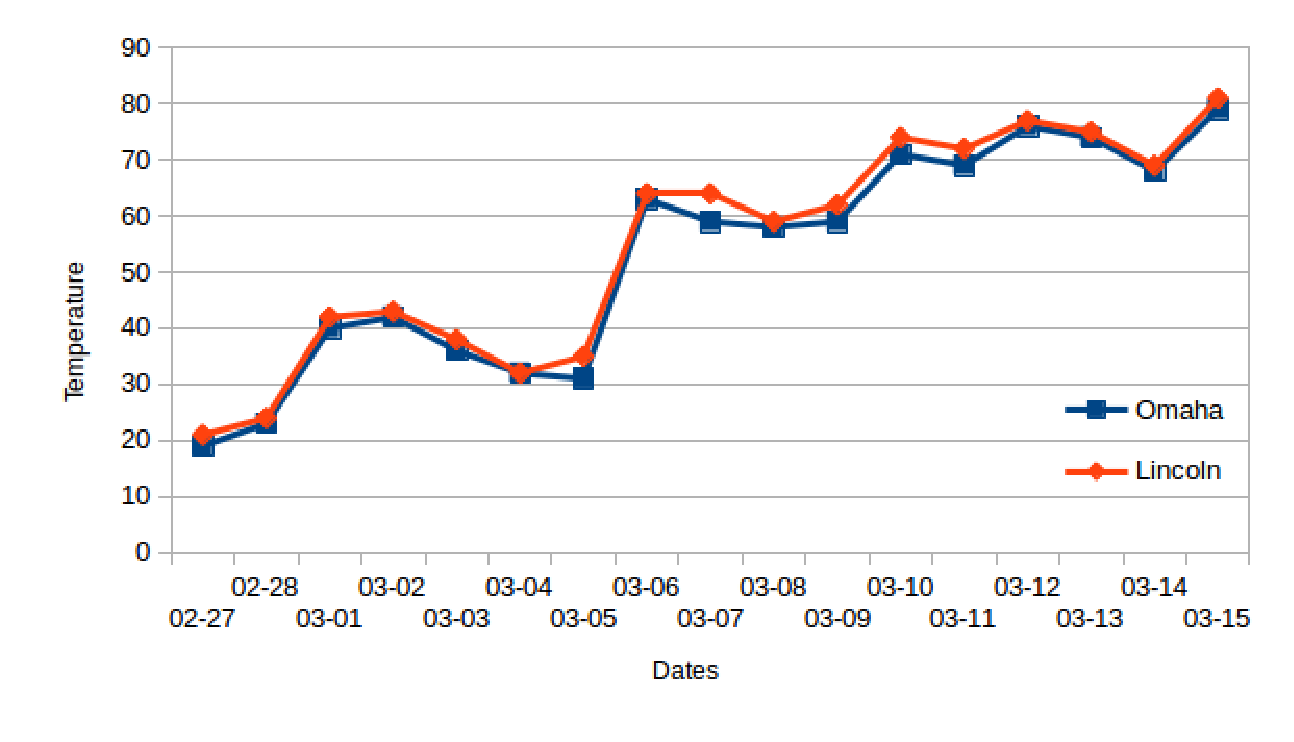
\includegraphics[scale=0.25]{chart1}}\quad
  \subfigure[Sentiment of Omaha and Lincoln Tweets]{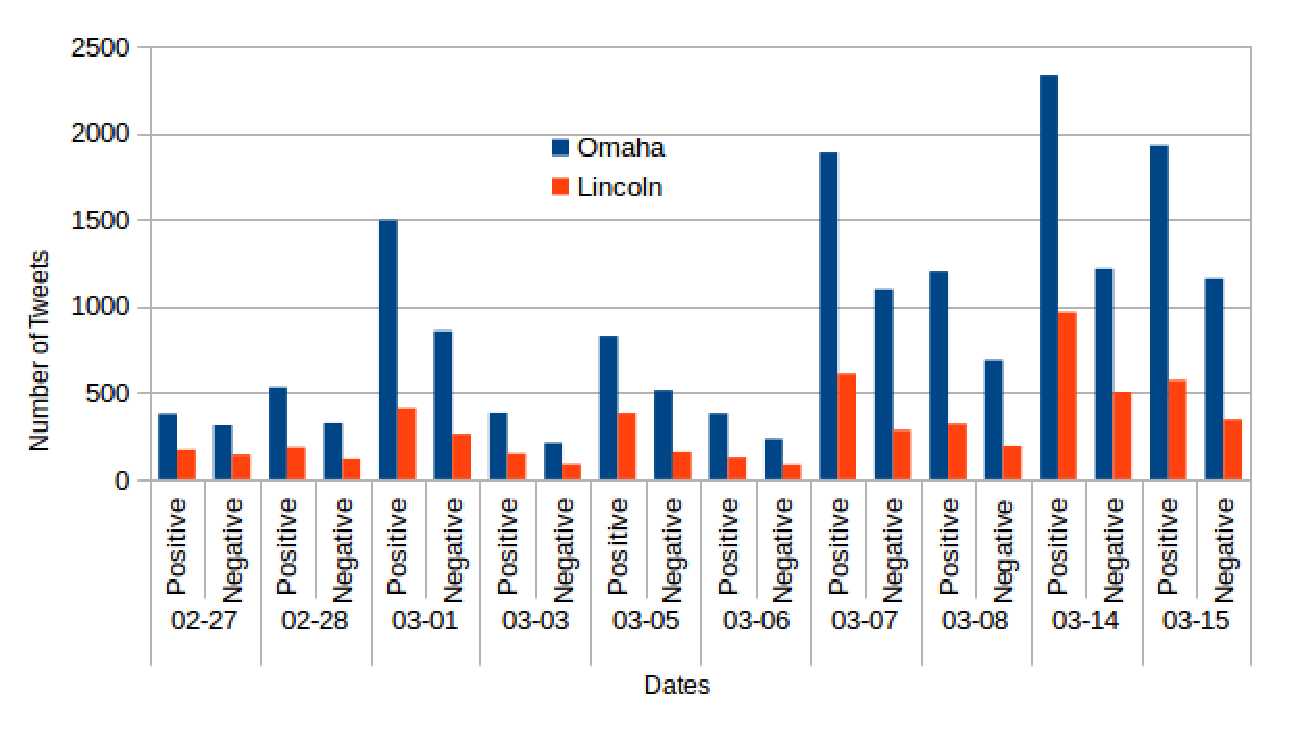
\includegraphics[scale=0.25]{chart2}}\quad
  \subfigure[Sentiment of Omaha and Lincoln Tweets]{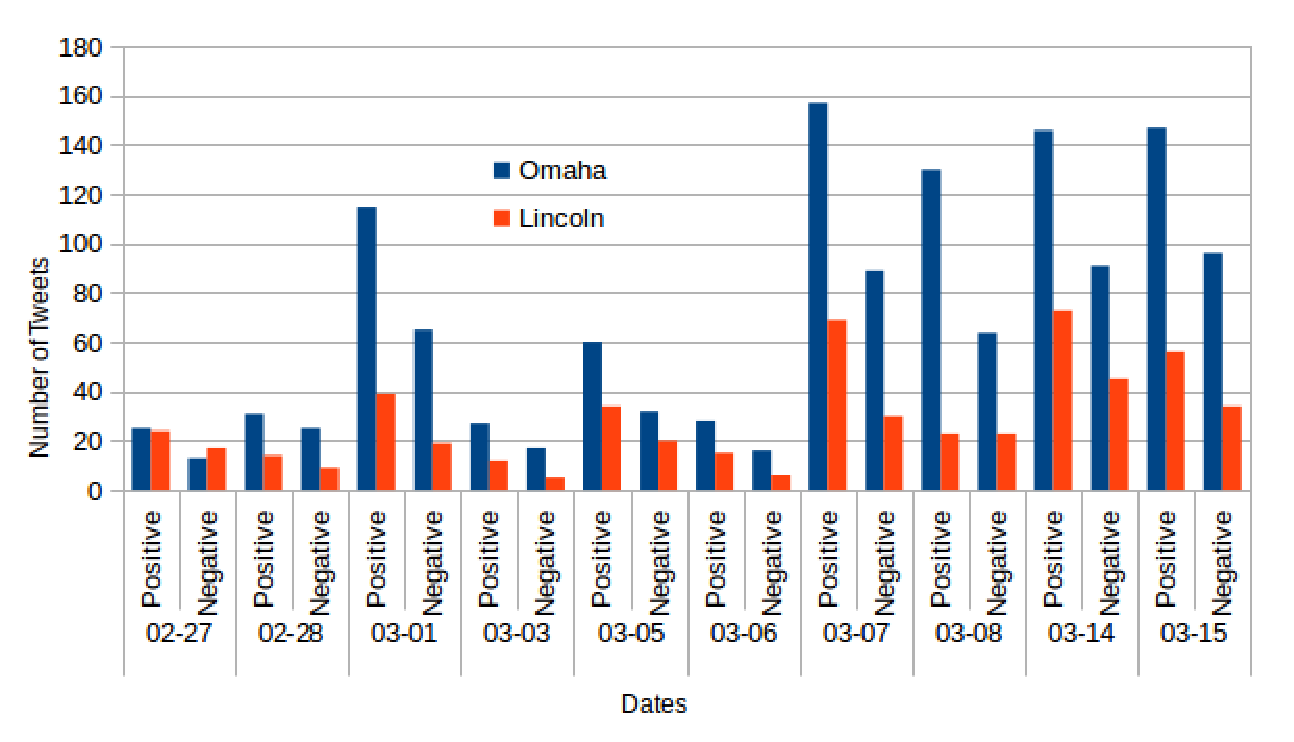
\includegraphics[scale=0.25]{chart3}}
\caption{The comparison of weather to sentiment.}
\label{fig:chart_1}
\end{figure*}

\section{Case Studies}
For our work, we have two goals. We first want to determine if there is any correlation between weather and mood. Secondly we would like to determine if our predicted mood is correct. 

\subsection{Tweet weather correlation}
We use two data sets to show our visualization. Using weather and twitter data from two back to back weekends we see if there is any relationship between the temperature and the overall mood of people. We are lucky that the days we chose show warmer changes in weather. Being on the brink of Spring we predict that the overall Tweets for the warmer weekend will have a more positive sentiment in comparison to the colder weekend. This weather pattern also can show any correlation we find for Seasonal Affective Disorder.

\subsubsection{All Tweets}
Of all the cities, we see that Omaha and Lincoln have the most tweets, so we will use these two cities to display our results. The weather patterns of the two weekends are shown in Figure \ref{fig:chart_1}(a). As seen in the figure, we choose to look at times where most of the population is awake (i.e. noon to 11 PM). From Figure \ref{fig:chart_1}(b) we can see the tweets and their sentiment for select days through the two weeks, where more emphasis is placed on the first week and less on the later. Each date has a positive and negative count, where we see that the pattern throughout is that the positive tweets outweigh the negative tweets. Another pattern that we see is that as the temperature increases the number of tweets increase however we see that more people tweet on Saturday than on Sunday. We think that this has to do with a number of factors; people go to church on Sunday where they choose to be among family, they do work around the house, or they don't have any eventful things which they feel they need to share. 

We do not see that with the change of temperature that there is a clear trend of more positive tweets versus negative tweets. The number of positive tweets is at least half the amount of negative tweets. The only item that we could see which may be weather related is that the amount of negative tweets is percentage wise far more in the colder temperatures in comparison to the warmer temperatures. In lieu of not finding any clear results, we look at tweets only with words related to weather to see if we find any trends.



\subsubsection{Weather related tweets}
Other than using all the tweets we collected we filter the collected tweets for weather-related terms. (i.e. snow, sunny, warm, cold, rain, etc.) We wanted to see if there was a stronger correlation in this situation compared to using all the tweets collected. In this situation, we are unfortunately limited to a few tweets. As we see in Figure \ref{fig:chart_1}(c) we see that the number of tweets drastically reduces to at most slightly less than 160 tweets for one day. 

Fortunately, we are able to see a pattern with weather and positive tweets. There is a spike of tweets when there is warmer weather. This pattern is seen in both sets of tweet data sets. However, we are now able to confirm that the correlation is due to weather. As the weather increased slightly on March 1st we see a spike in amount of tweets overall(Figure \ref{fig:chart_1}(b)) and also when the tweets had weather-related words(Figure \ref{fig:chart_1}(c)). We can also see that in Figure \ref{fig:chart_1}(c) that with the warmer weather the number of tweets in relation to the weather increased by approximately twice the amount. We still see the trend of more positive tweets in comparison to negative tweets when using the filtered data set.

\begin{figure}[htb]
 \centering
 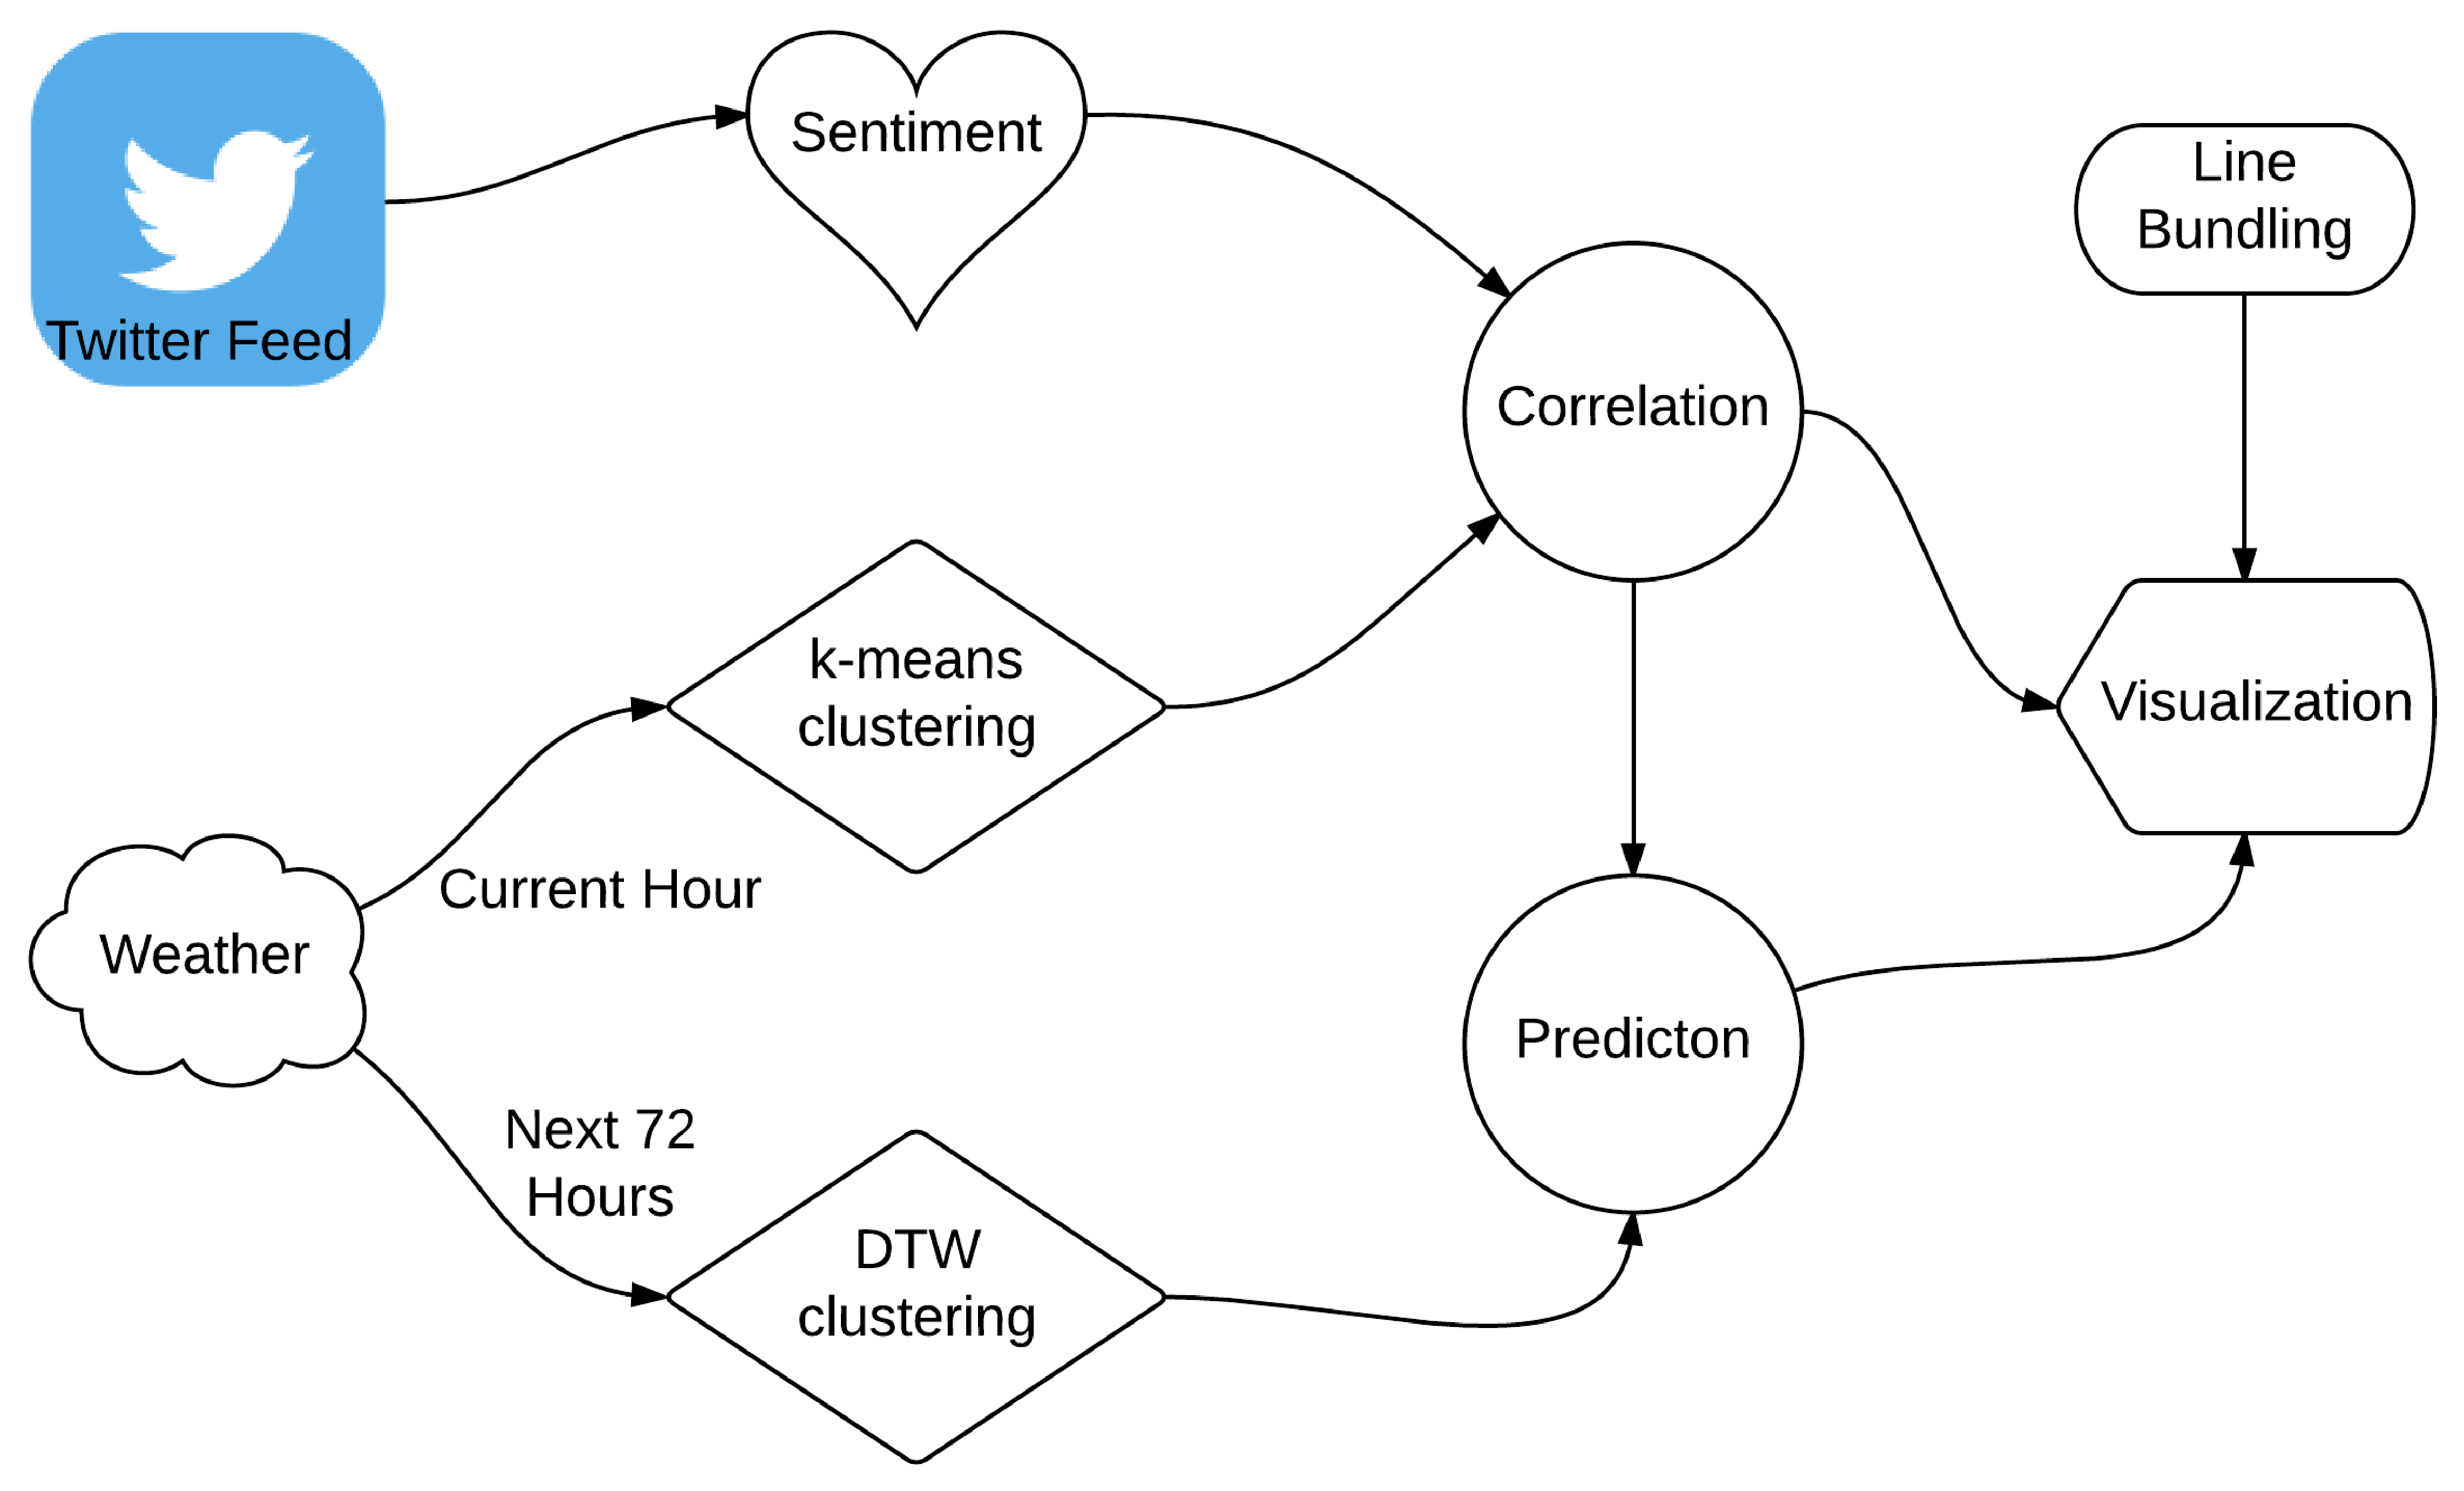
\includegraphics[scale=0.1]{steps}
 \caption{Accuracy of the different prediction methods}
 \label{fig:predict}
\end{figure}

\subsection{Predicted?}
Using the same data set we select a subset of two weekends to determine if the predicted value was close to the outcome. We chose March 6th, 7th and 8th for weekend one and March 13th, 14th and 15th for weekend two. The first weekend has between 10 to 20 degrees difference to the second weekend to take into account any change of weather patterns. We collect our predictions from Saturday and Sunday and compare them to the real sentimet of each hour. Again we focus on the two most populous cities in Nebraska; Lincoln and Omaha.

As we see in Figure \ref{fig:predict} the accuracy of the three methods we used are shown. 


\newpage


\section{Discussion}
We used a large data set to determine if there was any noticeable correlation, and we filter the data set to determine if this could provide a better indication of correlation. We saw that most of the tweets were positive in colder and warmer temperatures, however the number of tweets increased as the temperature rose. We observed the number of positive tweets percentage wise was much higher when the temperature rose. Even though our initial aim was to find a distinct answer to the question: Does the weather affect mood?, we were not able to gain concrete results. We were able to find other patterns from our analysis. 

Our bundling methods created smooth curves to create an aesthetic design. ....

We were able to determine the possible sentiment of users in select regions, even with lower a population. The results show ......

Correlating tweets to weather patterns is not a trivial task and requires multiple steps which can create errors at each step. Having a multi-step process the chance of error from classification can occur. 

There are a few items in regards to tweets that enforces a limit as to what we can assess. One drawback from tweets is that with a state population as small as Nebraska the chance of a user with their location enabled is minute. This dractically limits the amount of tweets we can attain each hour. Another limitation in some situations is tweet length since this may cause the complete expression of a user's feelings to be curbed. Other than Twitters limits we need to examine the suppressed feelings of users. Since Twitter is a social media hub, the need to express oneself in 140 characters may place a mask to what the user may be feeling. As proposed before there is no distinct way to determine the true feelings of a person.[3] Due to this phenomena we proposed the usage of only weather related tweets, due to there being a low chance of users masking their emotions. Even with this we saw that the majority of users use their tweets in a positive manner, so to expect a negative tweet is cynical in some sense.

Classifying the sentimet always brings error. Humans aren't known to be the most accurate at identify the sentiment of written statements. \cite{pangthumbs} When bringing in our own classifier, we believe that it can be improved. There are always certain words that can make the sentiment have a positive value instead of negative. Tweets are known to have sarcasm in them to introduce a form of satire or irony. \cite{riloff2013sarcasm} In situations like this there are some misclassifications of sentiment.

We believe that using the current weather limits us on other seasons which are approaching. So far we have experienced winter and spring weather. When we have the change of seasons its easy to see that there is some correlation with SAD. Like most of the population, the end of winter brings new changes, and thus new feelings. However, we don't know how the sentiment will change when summer, fall, or winter approaches. Nebraska is known for its intense heat and harsh winters, but these seasons also entail vacations and family gatherings. Analyzing these things can also provide more insight regarding our data sets, and what other filtering processes we may need.

\section{Future Work}

The future of this research can be expanded immensly. There are various aspects we can add to the existing work, or even alter the existing work. For altering existing work we would like to in the future make a cleaner looking visualization. Currently, there seems to be some rigidness to the design where corners could be smoothed have a clearer indication of what places link up to where. We also feel that we can make the design more intuitive without adding additional elements. Other than visualization we would like to implement a better sentiment classifier. Just by polling more tweets and gaining information regarding new words, determining sarcasm, irony, or satire, and finding new linguistic patterns we believe we can gain a better classifier. Additionally we would also like to improve the sentiment prediction.

For supplementing this work we have a few items which we believe we can add. This work as of now only sees the relation to temperature, but this study could be extended to be applied to precipitation, humidity, wind speed, or any other weather variables. There may be a significant correlation between rain amount and negative tweets. As we approach warmer climates we can conduct research regarding what the overall sentiment of people to rain, storms, and strong wind conditions. We also believe that we can determine if there is a better correlation of weather to other variables, possibly ones which are directly impacted by weather such as road accidents, calamities from natural disasters, or even medical episodes like the flu. Since there is no real way to determine if a person's mood is truly affected by weather we think using some other variables can provide more concrete correlation results. 

This work can be expanded to other states and see if in more populous states the outcome would be more different. We also think that states which don't experience much seasonal change will have very different outcomes and not reflect any correlation between weather patterns and sentiment.



\section{Conclusion}

In this paper, we introduced Tweether, a visualization tool for displaying the correlation of weather to tweets. Other than making a novel visualization to showcase correlation between weather and sentiment our main goal was to determine if there was any correlation between usage of social media and weather patterns. Using two data sets, we were able to determine that there is some correlation with the amount of tweets related to weather when it is warm in comparison to the colder weather. 

Visualizations showcasing social media sentiment has been done many times before, and similarly clustering of weather has been implemented numerous times before. However, there have been few to none works out there which try to find the correlation between the two. 

We realized that this work can be expanded to apply to many different scenarios, but we chose to apply it to a question that has been asked for centuries. ...

Our prediction technique worked for...

The line bundling implemented in this visualization is an entity on its own and should be applied to many different works. ...




%% if specified like this the section will be committed in review mode
\acknowledgments{
The authors wish to thank A, B, C. This work was supported in part by
a grant from XYZ.}

\newpage


\bibliographystyle{abbrv}
%%use following if all content of bibtex file should be shown
\nocite{*}
\bibliography{template}
\end{document}

